
\chapter{Data analysis} \label{data-analysis-chapter}
\subsubsection{Kenward cattle weight data}

\cite{kenward1987method} reported an experiment designed to investigate the impact of the control of intestinal parasites in cattle. The grazing season runs from spring to autumn, during which cattle can potentially ingest roundworm larvae which develop from eggs deposited around the pasture from feces of previously infected cattle. Once infected, the animal is deprived of nutrients and immune resistance to disease is suppressed which can significantly impact animal growth. Monitoring the effect of a treatment for the disease requires repeated weight measurements on animals over the grazing season. 

\bigskip

To compare two methods for controlling the disease, say treatment A and treatment B, each of 60 cattle were assigned randomly to two groups, each of size 30. Animal subjects were put out to pasture at the start of grazing season, with each member of the groups receiving one of the two treatments. Animals were weighed $p = 11$ times over a 133-day period; the first 10 measurements on each animal were made at two-week intervals and the final measurement was made one week later. Weights were recorded to the nearest kilogram, and measurement times were common across animals. The longitudinal dataset is balanced, as there were no missing observations for any of the experimental units. Observed weights are shown in Figure~\ref{fig:cattle-weights-by-trt}.

\begin{center}  
\begin{figure}[H] 
\begin{center}
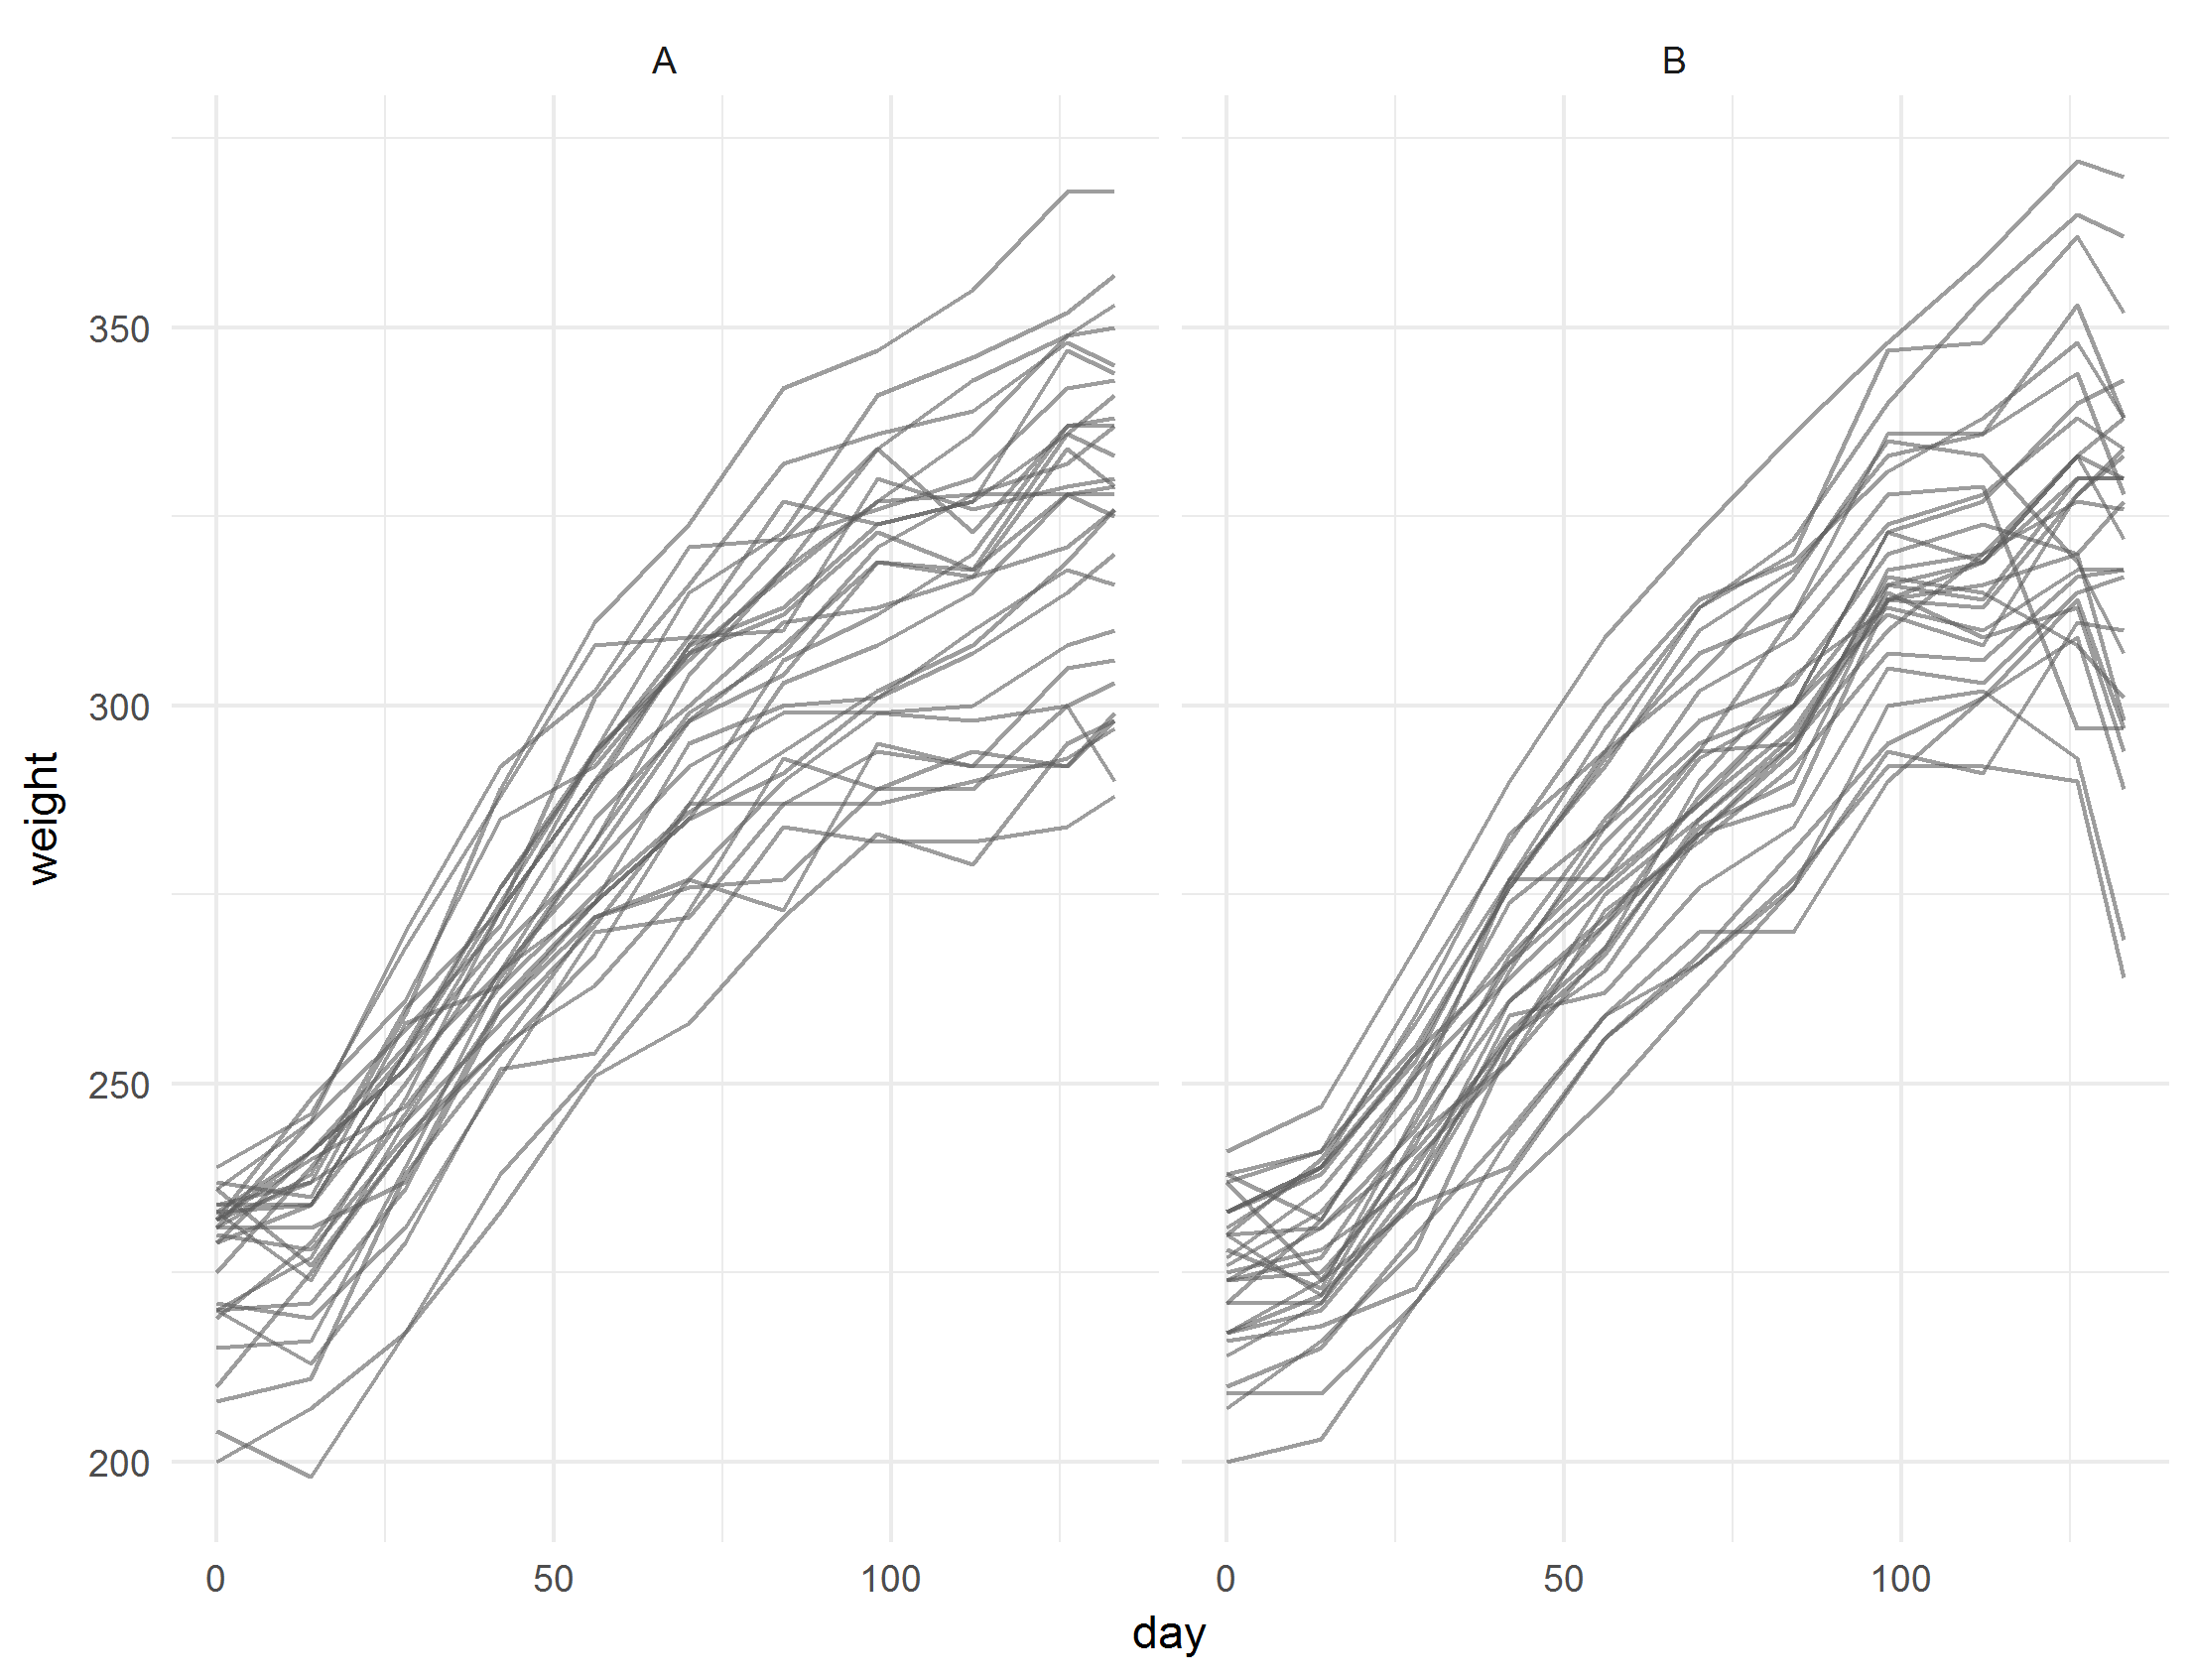
\includegraphics[width = 1.1\textwidth, height = 5in]{img/cattle/cattle-weights-vs-time-by-trt}
\caption{\textit{Subject-specific weight curves over time for treatment groups A and B.}}\label{fig:cattle-weights-by-trt}
\end{center}
\end{figure} 
\end{center}

We see an upward trend in weights over time, with variance in weights increasing over time for both groups. Treatment group B demonstrates a sharp decrease in the final weight measurement. The analysis of the same dataset provided by \cite{zimmerman1997structured} rejected equality of the two covariance matrices corresponding to treatment group using the classical likelihood ratio test, making it reasonable to study each treatment group's covariance matrix separately. Following \cite{pan2017jmcm}, \cite{zhang2015joint}, and \cite{pourahmadi1999joint}, we analyze the data from the $N = 30$ cattle assigned to treatment group A, which we assume share a common $11 \times 11$ covariance matrix $\Sigma$. The left profile plot in Figure~\ref{fig:cattle-weights-by-trt} of the weights for units in treatment group A shows a clear upward trend in weights;  variances appear to increase over time, suggesting that the covariance structure is nonstationary.

\bigskip

The nonstationarity suggested in Figure~\ref{fig:cattle-weights-by-trt} is also supported by the sample correlations given in Table~\ref{table:cattleA-sample-correlations}; correlations within the subdiagonals are not constant and increase over time, a secondary indication that a stationary covariance is not appropriate for the data.  Table~\ref{table:sample-regressogram-garps} gives the sample generalised autoregressive parameters and the innovation variances, which are plotted in Figure~\ref{fig:cattleA-regressogram} and Figure~\ref{fig:cattleA-innovation-variogram} respectively. 

\begin{table}[H] 
\begin{center}
\begin{tabular}{r|rrrrrrrrrrr}
& \multicolumn{11}{c}{day}\\
&&&&&&&&&&\\
& 0 & 14 & 28 & 42 & 56 & 70 & 84 & 98& 112& 126 &133\\
  \hline\noalign{\smallskip} 
0 & 1.00  \\ 
  14 & 0.82 & 1.00  \\ 
  28 & 0.76 & 0.91 & 1.00 & \\ 
  42 & 0.65 & 0.86 & 0.93 & 1.00 &  \\ 
  56 & 0.63 & 0.83 & 0.89 & 0.93 & 1.00 &  \\ 
  70 & 0.58 & 0.75 & 0.85 & 0.90 & 0.94 & 1.00 & \\ 
  84 & 0.51 & 0.64 & 0.75 & 0.80 & 0.85 & 0.92 & 1.00 &\\ 
  98 & 0.52 & 0.68 & 0.77 & 0.82 & 0.88 & 0.93 & 0.92 & 1.00 & \\ 
  112 & 0.51 & 0.61 & 0.71 & 0.74 & 0.81 & 0.89 & 0.92 & 0.96 & 1.00 & \\ 
  120 & 0.46 & 0.59 & 0.69 & 0.70 & 0.77 & 0.85 & 0.86 & 0.94 & 0.96 & 1.00 &  \\ 
  133 & 0.46 & 0.56 & 0.67 & 0.67 & 0.74 & 0.81 & 0.84 & 0.91 & 0.95 & 0.98 & 1.00 \\ 
   \hline
\end{tabular}
\caption{\textit{Cattle data: treatment group A sample correlations.}}\label{table:cattleA-sample-correlations}
\end{center}
\end{table}


\begin{table}[H] 
\begin{center}
\begin{tabular}{lc|ccccccccccc|cr}
 \multicolumn{14}{c}{day} \\
&&&&&&&&&&&&\\
& &  0 & 14 & 28 & 42 & 56 & 70 & 84 & 98 & 112 & 126 & 133  \\ 
  \cline{2-13}\noalign{\smallskip}  
&0 & 1 & &&&&&&&&& & 4.673& \\ 
&  14& 1.00 & 1&&&&&&&&&& 3.939 &\\ 
&  28 & 0.04 & 0.90 & 1 &&&&&&&&& 3.370&\\ 
&  42 & -0.25 & 0.25 & 0.88 & 1 &&&&&&&&3.000& \\ 
&  56 & -0.02 & 0.07 & 0.12 & 0.90 &1 &&&&&&& 3.299&\\ 
day &  70 & 0.04 & -0.28 & 0.11 & 0.37 & 0.82  &1&&&&&& 3.363 & $\log\left(\hat{\sigma}^2_t\right)$\\ 
 & 84 & 0.12 & -0.23 & 0.04 & -0.16 & 0.08 & 1.03  &1&&&&& 3.610\\ 
 & 98 & -0.06 & 0.05 & 0.02 & -0.27 & 0.23 & 0.61 & 0.42 &1&&&& 3.403&\\ 
 & 112 & 0.18 & -0.10 & 0.05 & -0.26 & -0.10 & 0.03 & 0.30 & 0.93&1&&& 2.780&  \\ 
 & 126 & -0.26 & 0.15 & 0.45 & -0.33 & -0.19 & 0.01 & -0.18 & 0.37 & 0.94 &1&&3.280& \\ 
 & 133 & 0.13 & -0.26 & 0.08 & 0.28 & 0.04 & -0.36 & -0.05 & -0.07 & 0.37 & 0.85 & 1  &2.262&\\ 
\end{tabular} 
\caption{\textit{Cattle data: treatment group A sample generalized autoregressive parameters (below the main diagonal) and log sample innovation variances (rightmost column).}}\label{table:sample-regressogram-garps}
\end{center}
\end{table}

\begin{figure}[H]
 \begin{subfigure}[t]{.65\textwidth}
  \centering
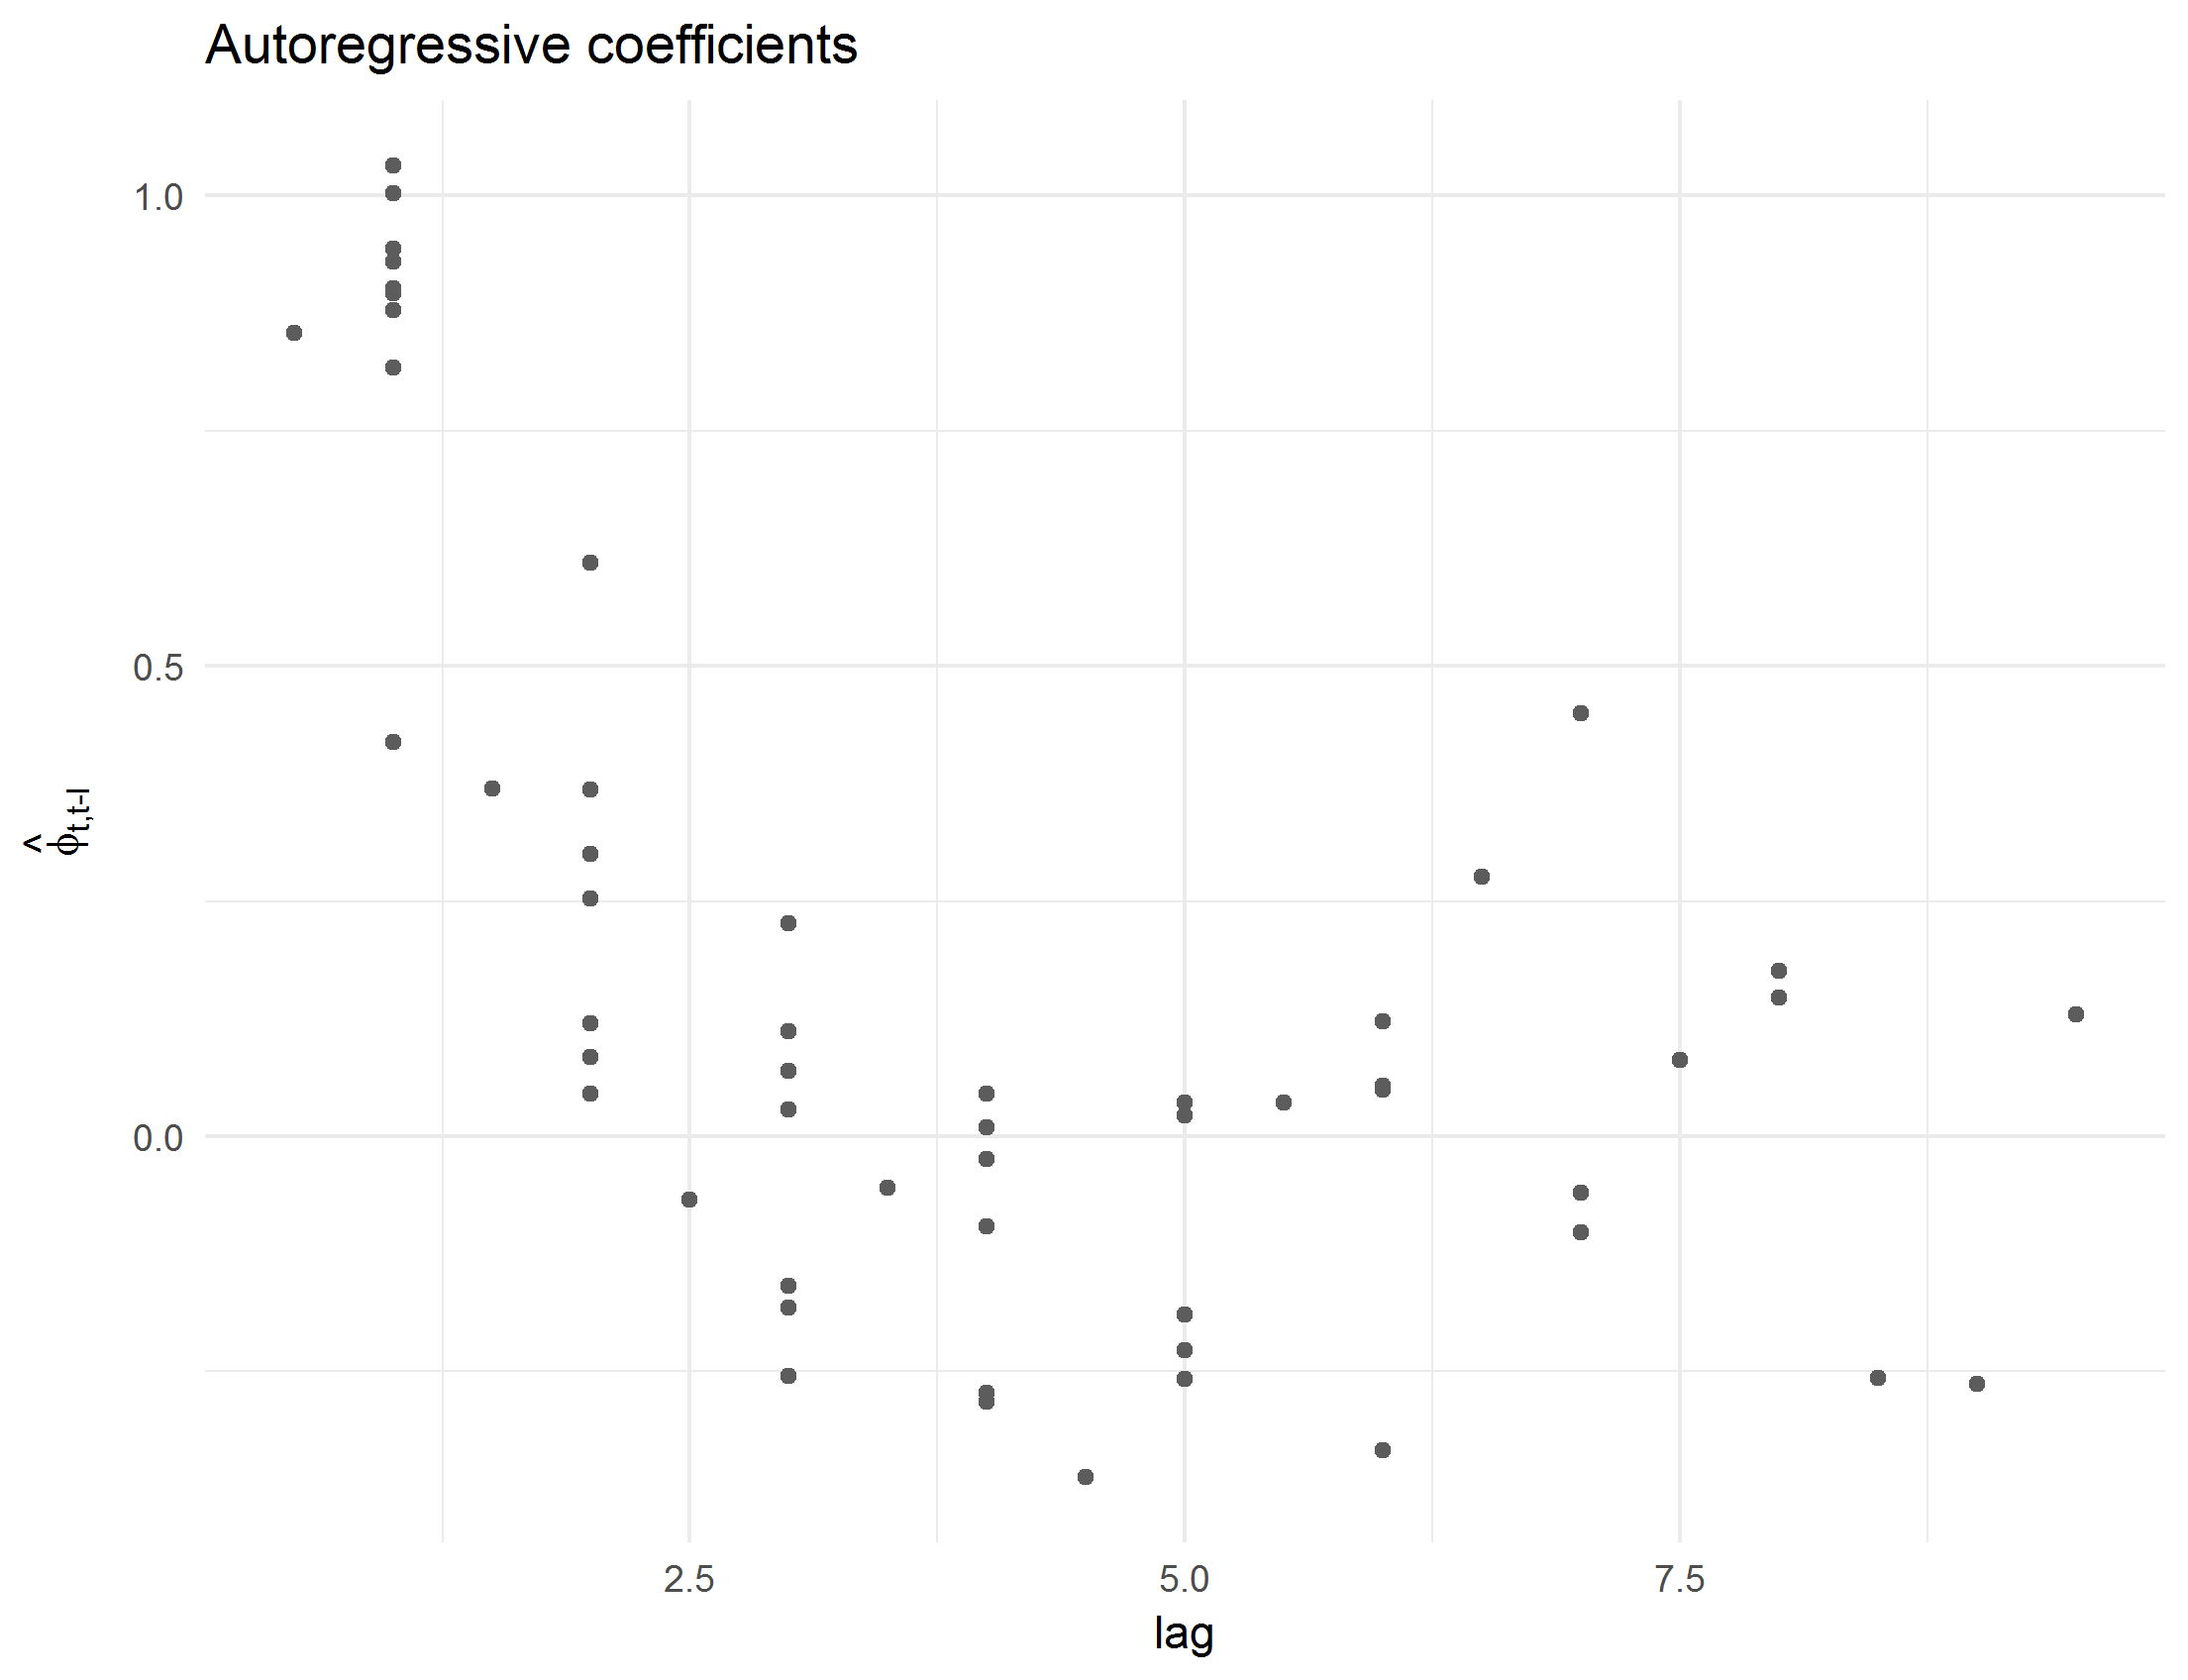
\includegraphics[width = \textwidth]{img/cattle/cattleA-regressogram}
 \caption{\textit{Sample generalized autoregressive parameters $\hat{\phi}_{ts}$.}}
\label{fig:cattleA-regressogram}
 \end{subfigure}
   \centering
    \begin{subfigure}[t]{.65\textwidth}
    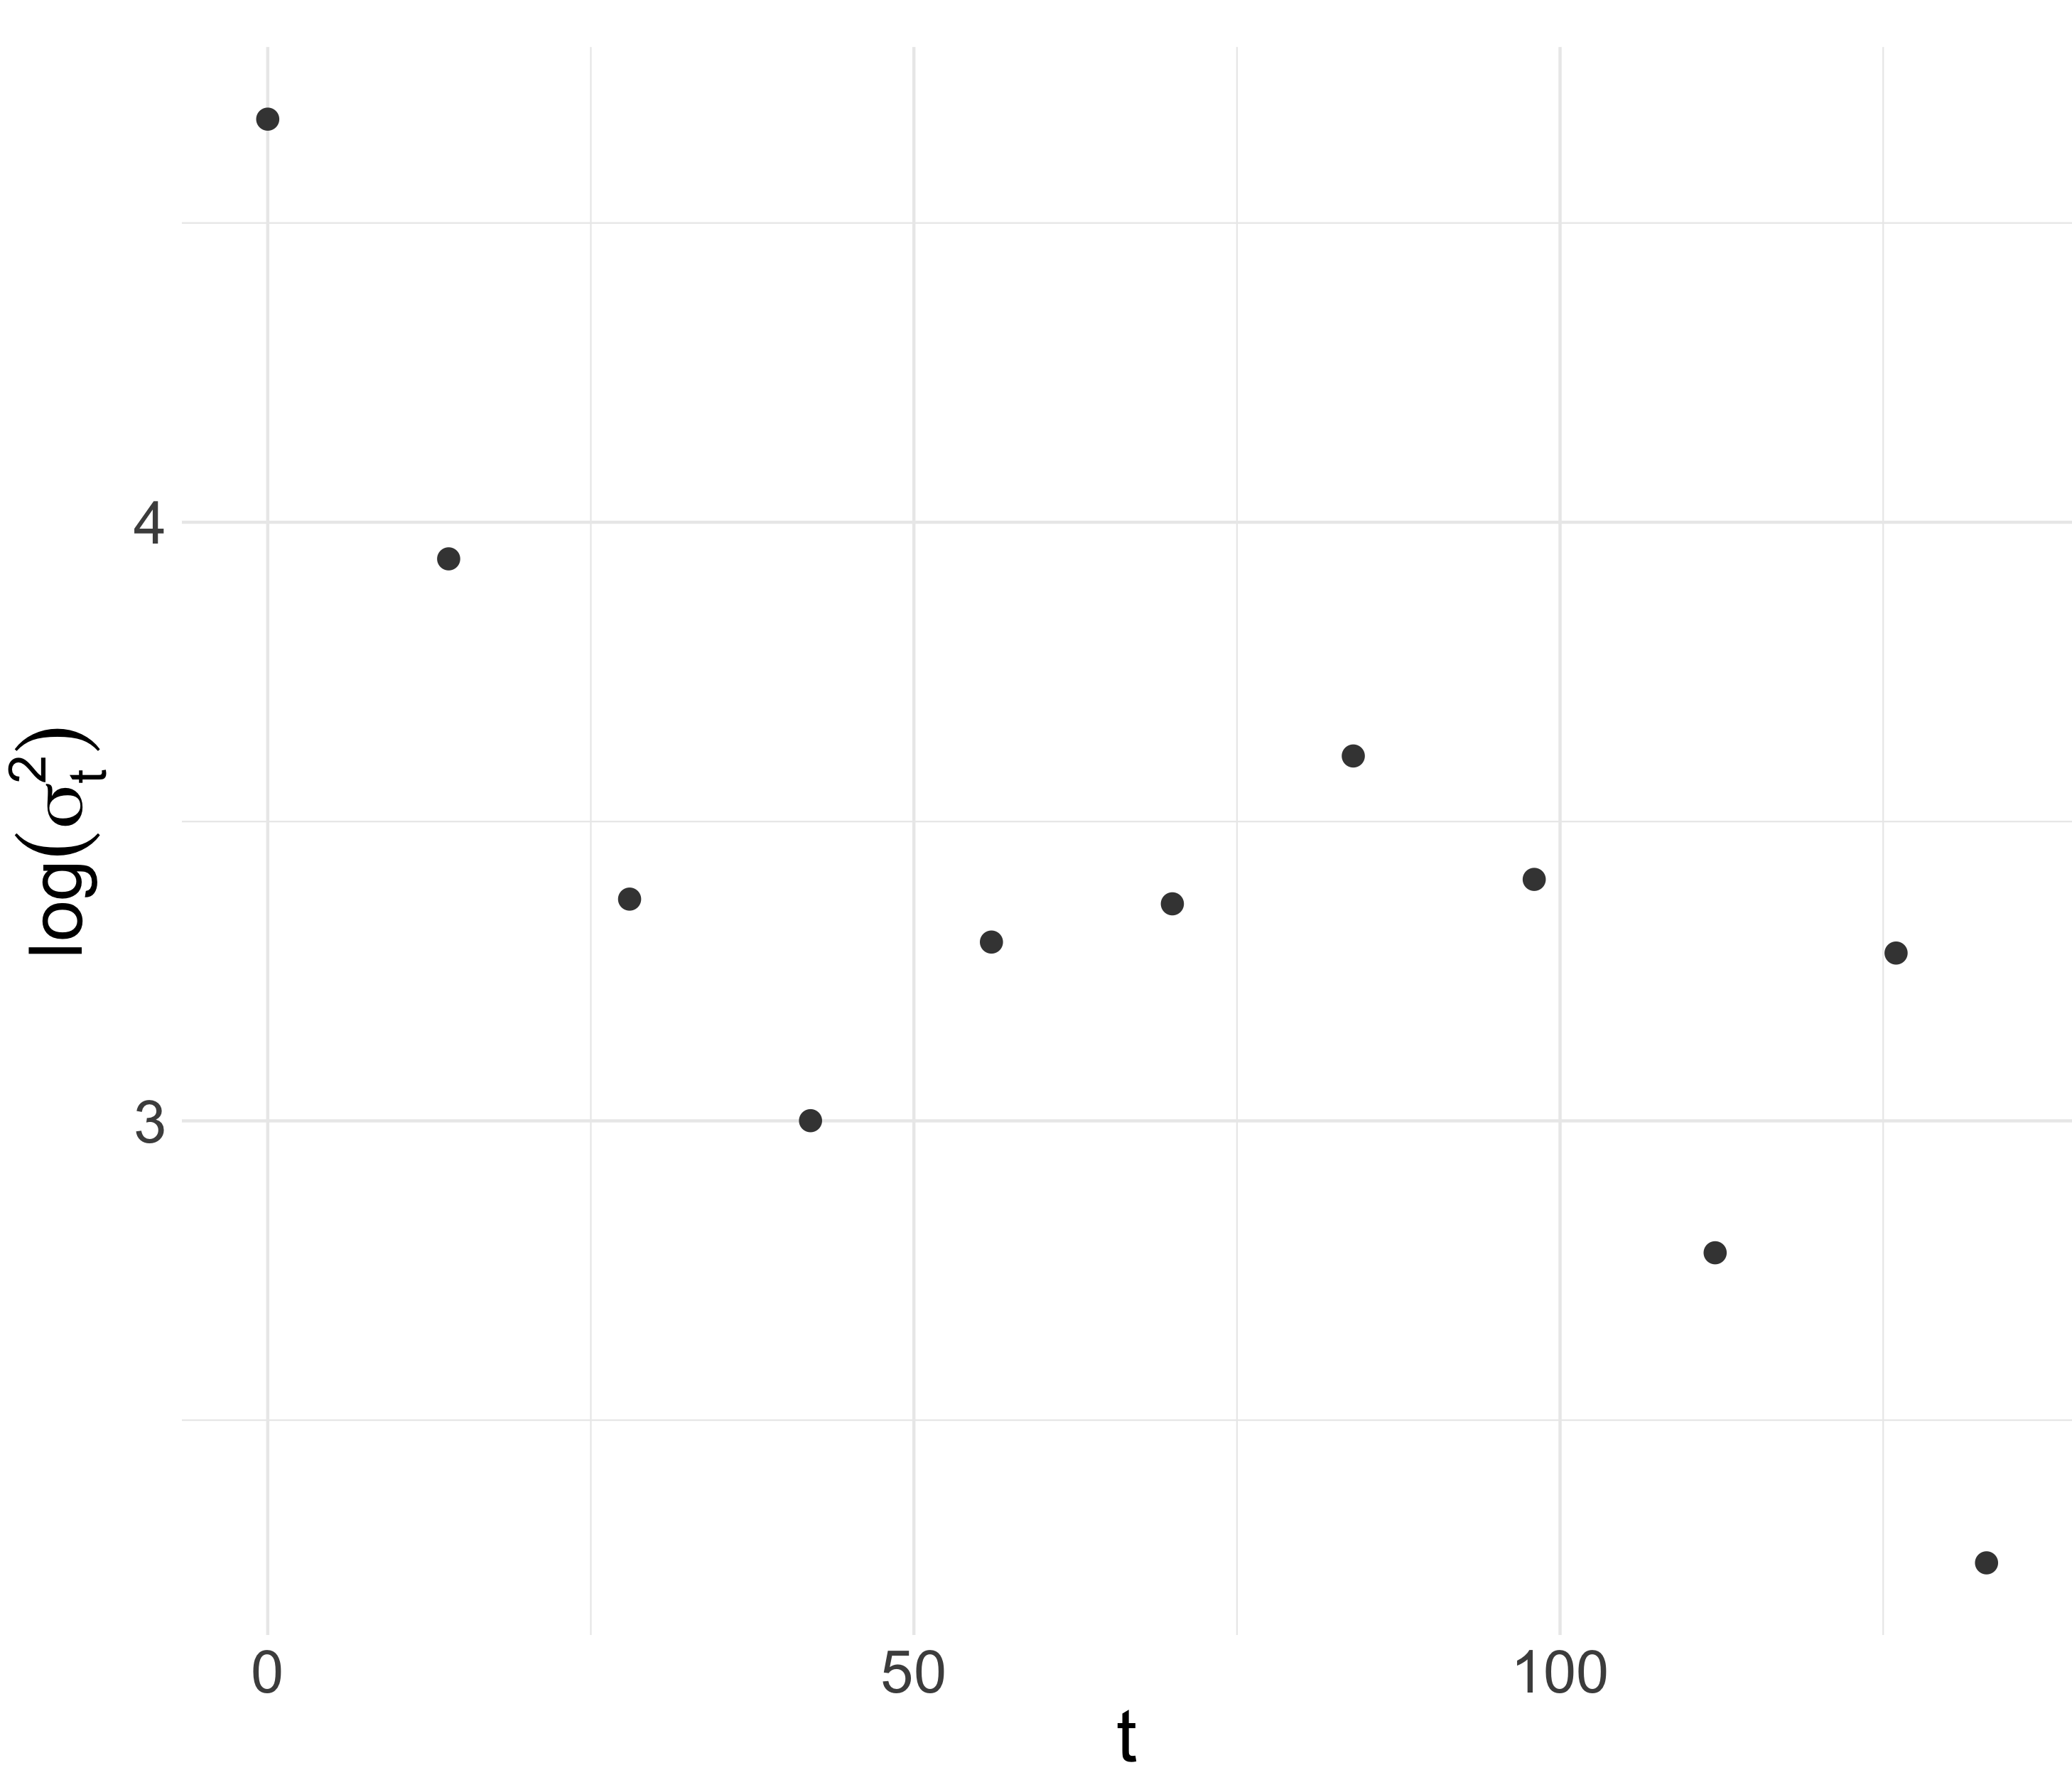
\includegraphics[width=\textwidth]{img/cattle/cattleA-innovation-variogram}
 \caption{\textit{Sample innovation variances $\hat{\sigma}_t^2$}} \label{fig:cattleA-innovation-variogram}
 \end{subfigure}
 \caption{\textit{Empirical estimates of the parameters of the Cholesky decomposition of the sample covariance matrix.}} \label{fig:cattleA-innovation-variogram-and-regressogram}
\end{figure}

%
%\begin{figure}[H] \label{fig:cattleA-innovation-variogram}
%\begin{center}
%    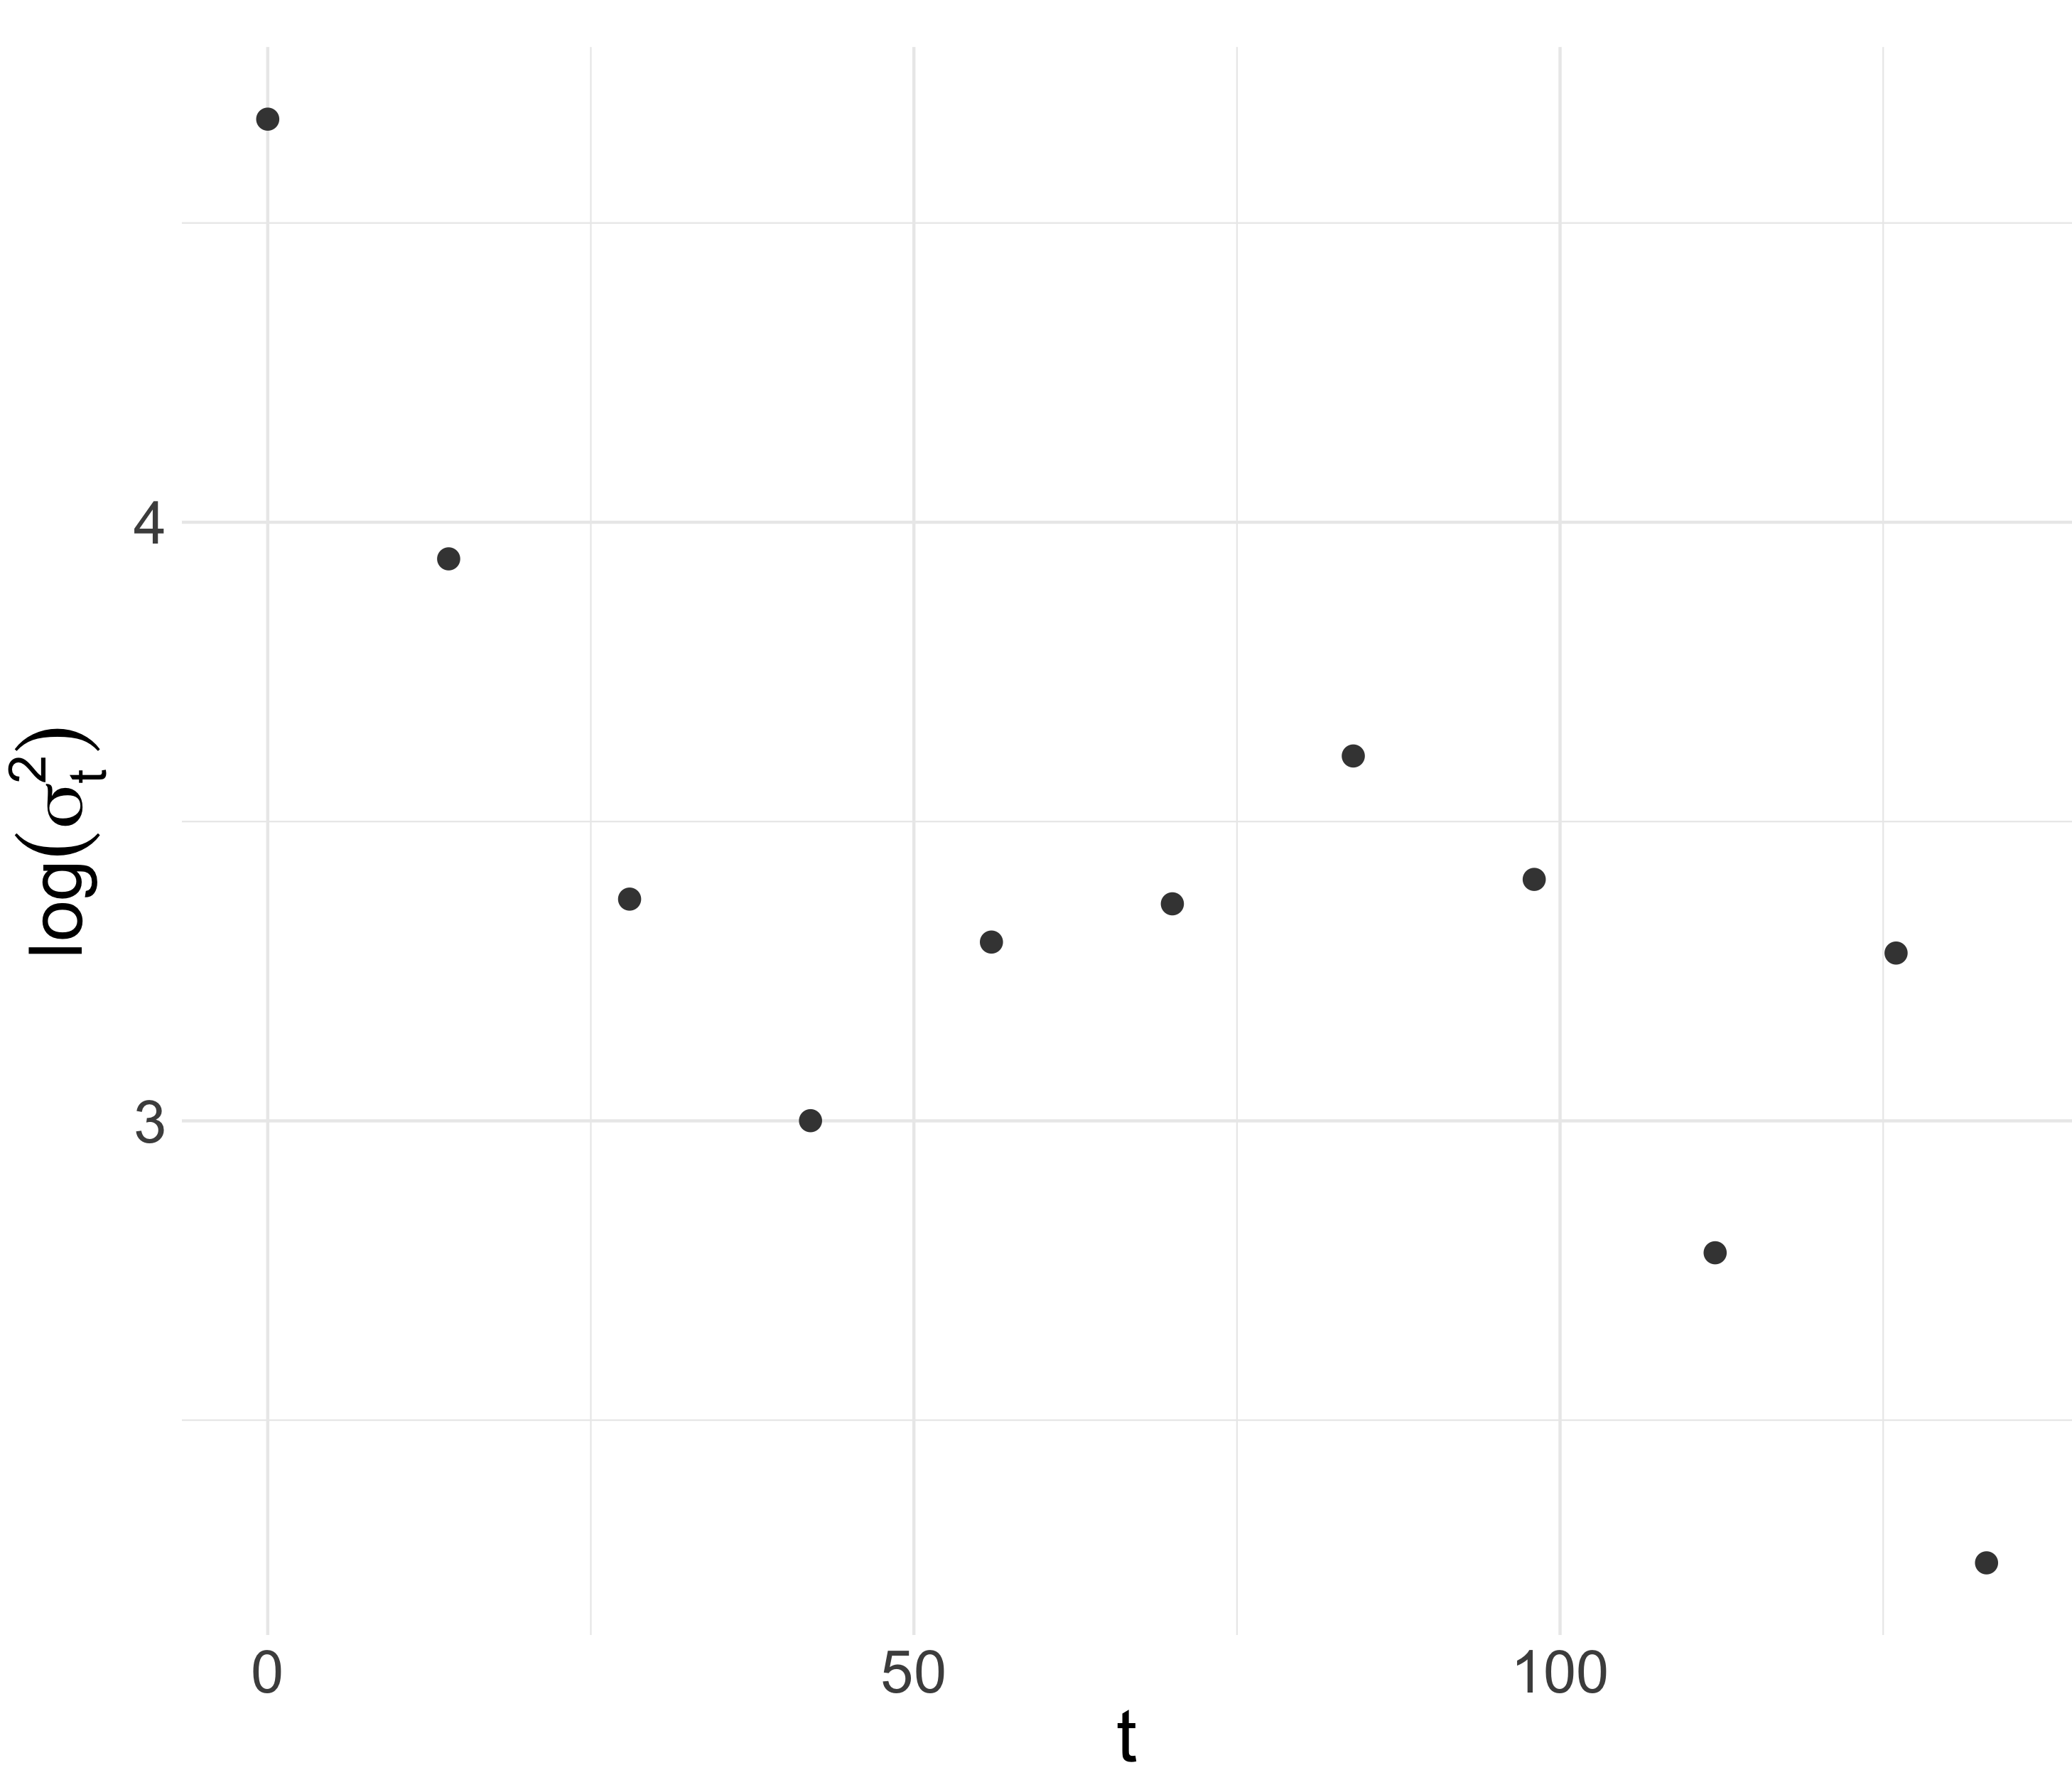
\includegraphics[width=\textwidth]{img/cattle/cattleA-innovation-variogram}
%\end{center}
% \caption{Sample estimates of innovation variances $\sigma_t^2$ obtained by applying the modified Cholesky decomposition to the sample covariance matrix.}
% \end{figure}
%
%\begin{figure}[H] \label{fig:cattleA-regressogram}
%\begin{center}
%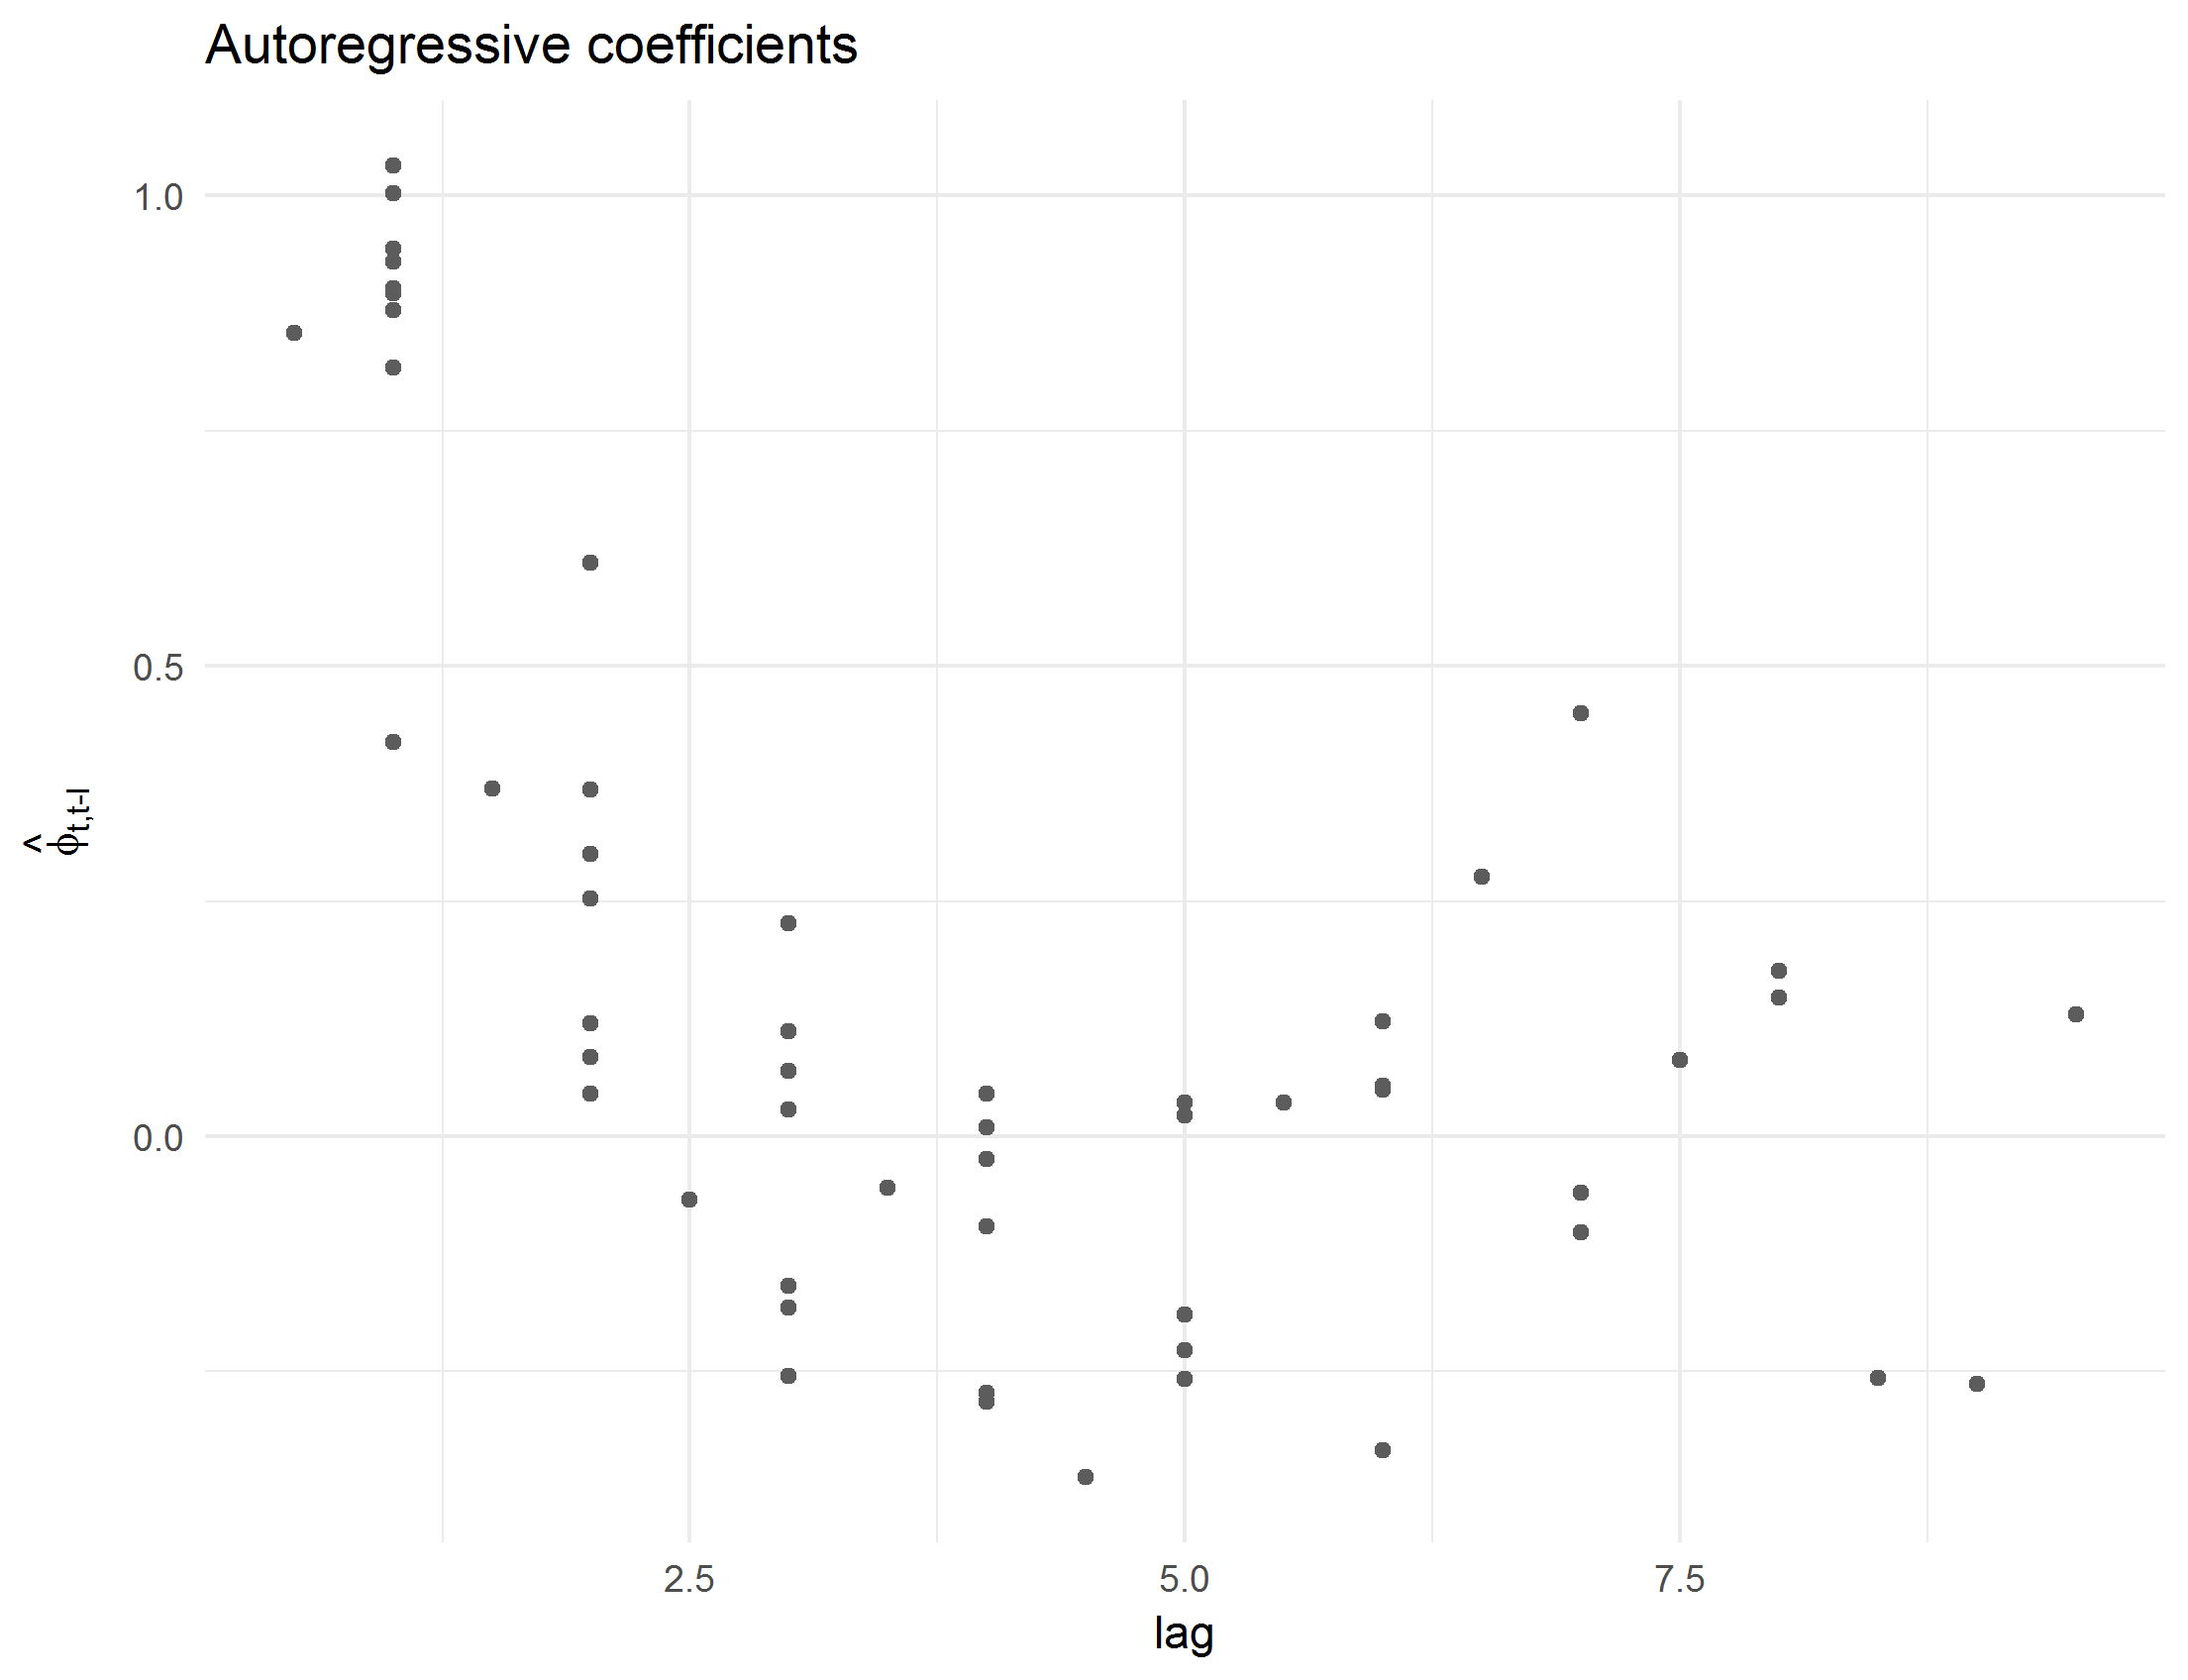
\includegraphics[width = \textwidth]{img/cattle/cattleA-regressogram}
%\end{center}
% \caption{Sample estimates of the generalized autoregressive parameters $\phi_{ij}$ obtained by applying the modified Cholesky decomposition to the sample covariance matrix.}
%\end{figure} 

Analyzing the sample regressogram (Figure~\ref{fig:cattleA-regressogram}) and sample innovation variogram (Figure~\ref{fig:cattleA-innovation-variogram}), \cite{pourahmadi1999joint} suggested that both sample generalized autoregressive parameters and the logarithms of the innovation variances can be characterized in terms of cubic functions of the lag only. They model 

\begin{align}
\begin{split} \label{eq:pourahmadi-cubic-model}
\phi_{ts} = x'_{ts}\gamma, \\
\log\left(\sigma_t^2\right) = z'_{t}\xi, 
\end{split}
\end{align}
\noindent
for $t = t_2,\dots, t_{11}$ where 

\begin{align*}
x'_{ts} = \begin{bmatrix} 1 & t - s& \left(t - s\right)^2 & \left(t - s\right)^3 \end{bmatrix},\; \mbox{and } z'_{t} = \begin{bmatrix} 1 & t& t^2& t^3 \end{bmatrix}.
\end{align*}
\noindent
They estimate $\gamma$ and $\xi$ via maximum likelihood.  Figure~\ref{fig:cattleA-smoothed-regressogram-variogram} shows the estimated cubic polynomials corresponding to Model~\ref{eq:pourahmadi-cubic-model}. 

\begin{figure}[H]
  \centering
 \begin{subfigure}[t]{.65\textwidth}
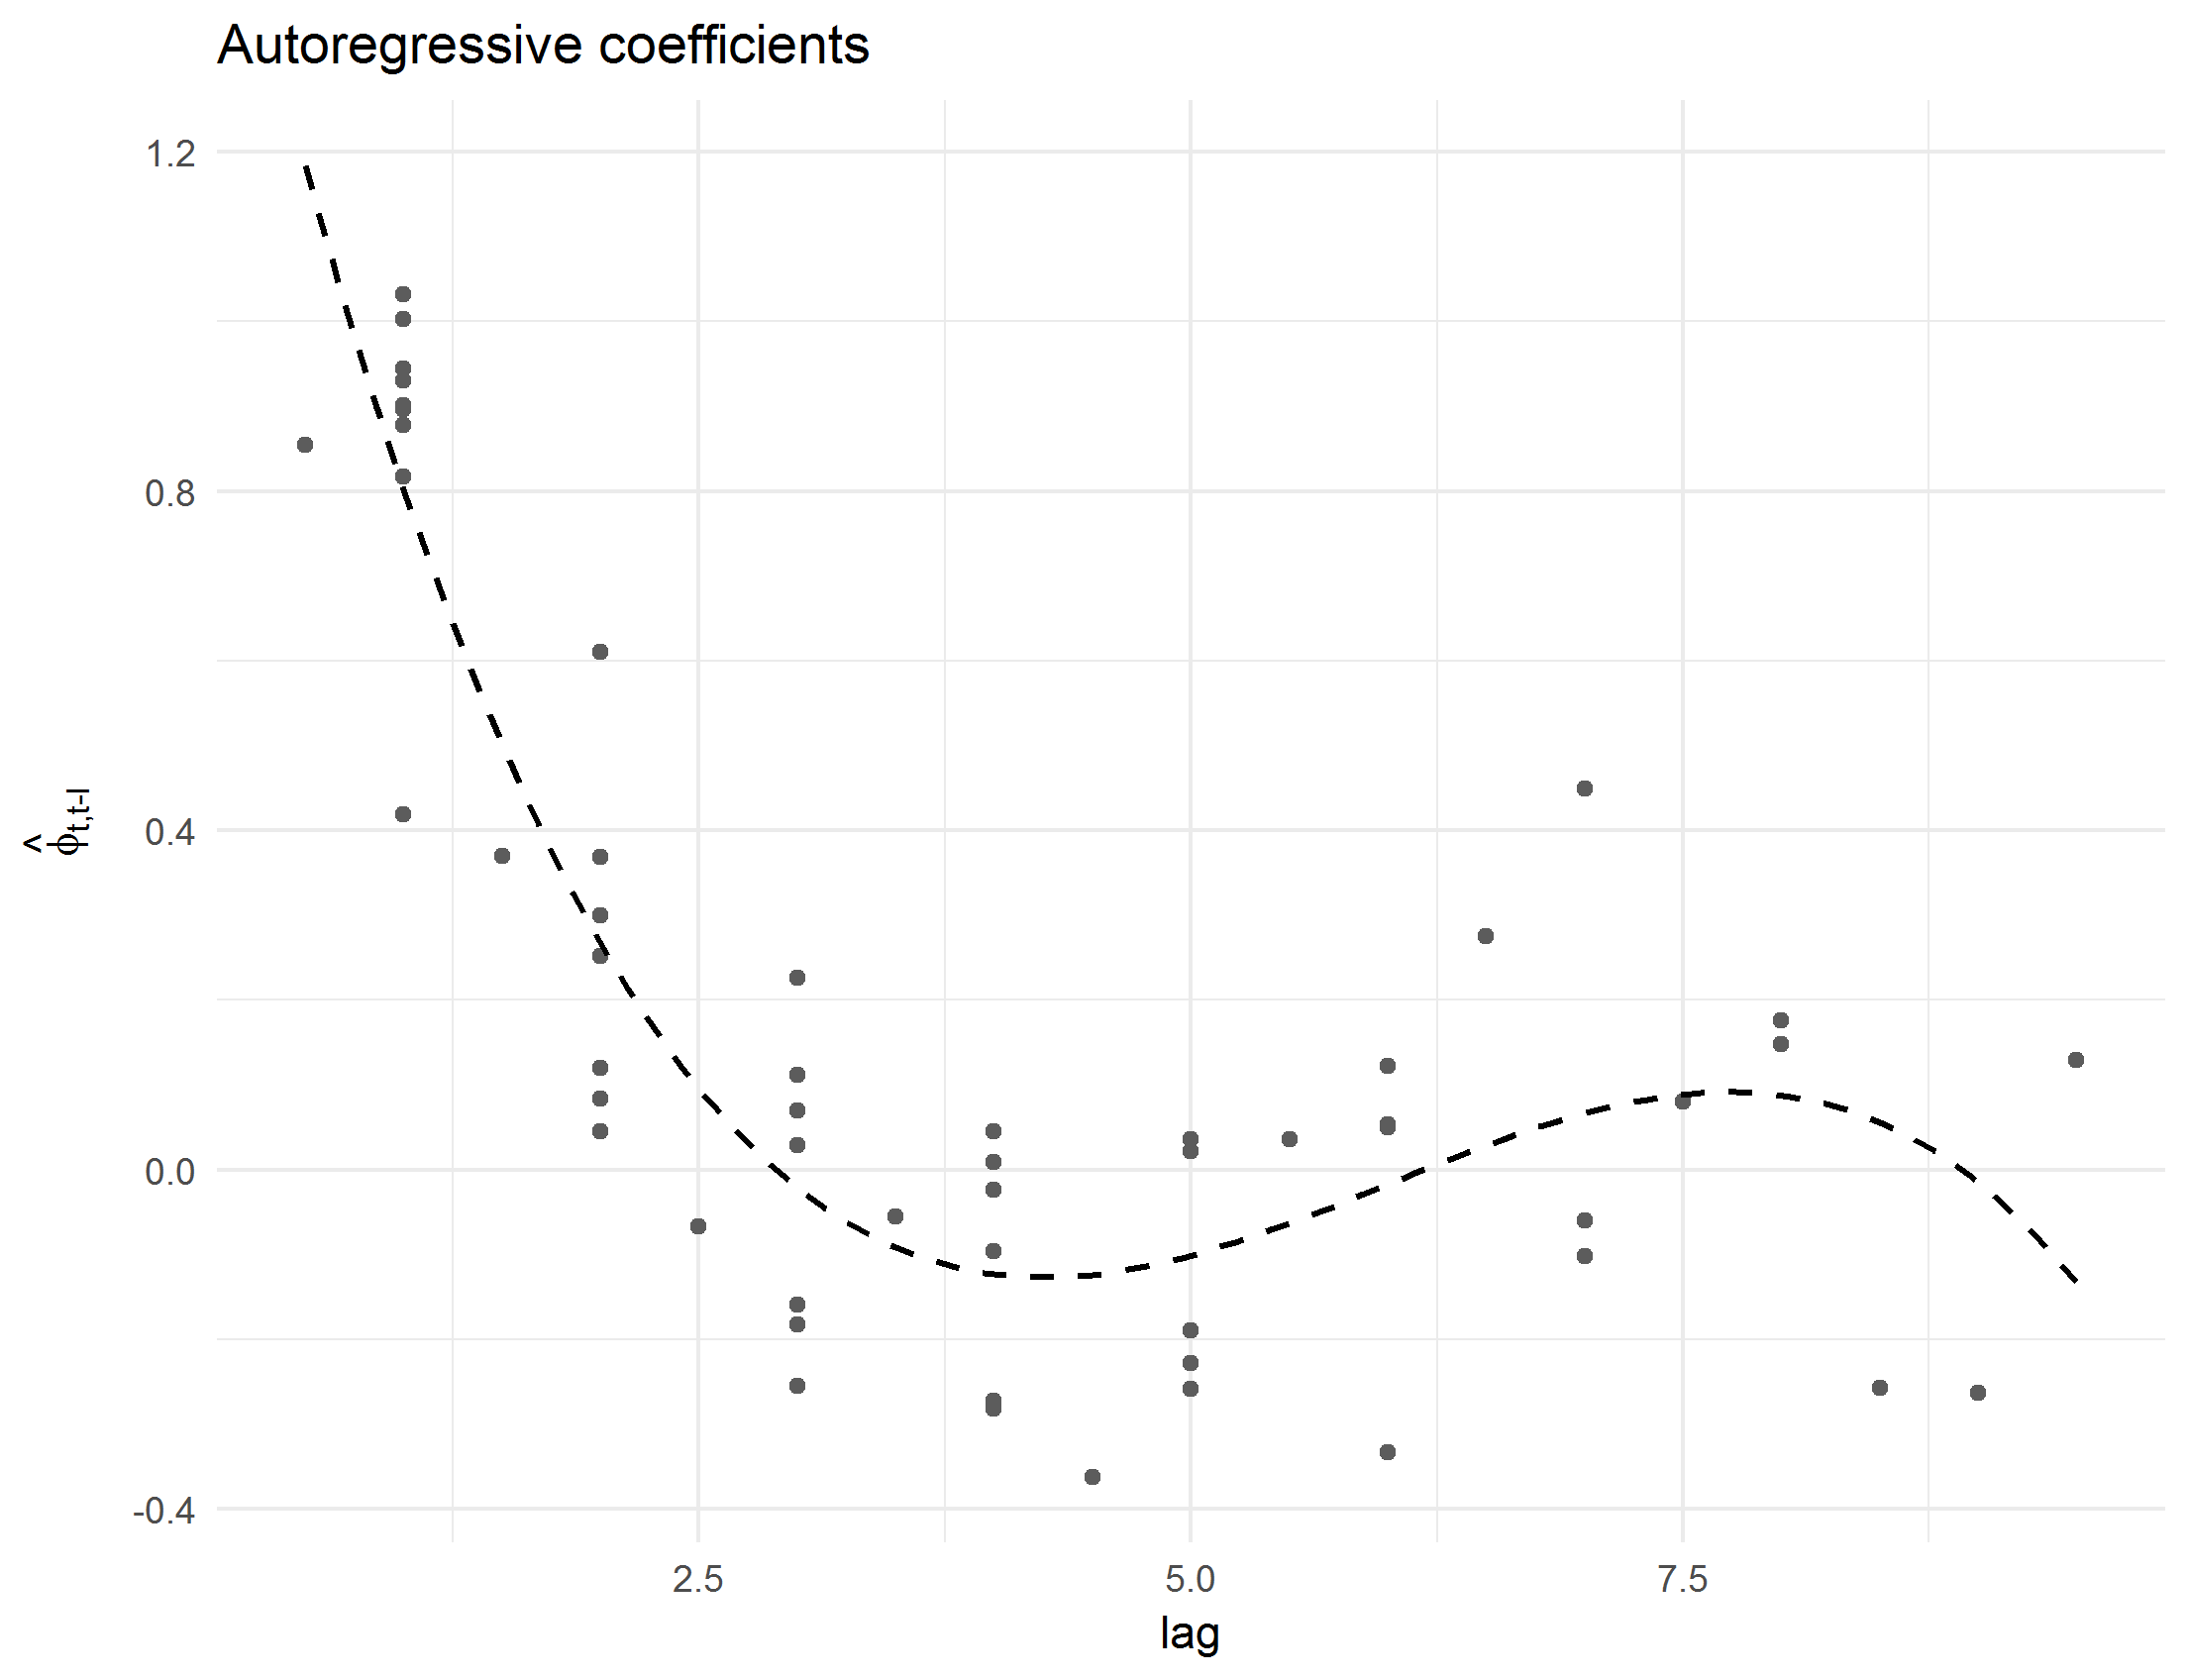
\includegraphics[width = \textwidth]{img/cattle/cattleA-regressogram-with-cubic-smooth}
 \caption{\textit{Smoothed sample regressogram.} }
 \label{fig:cattleA-innovariogram-with-cubic-smooth}
 \end{subfigure}
 \hfill
   \centering
 \begin{subfigure}[t]{.65\textwidth}
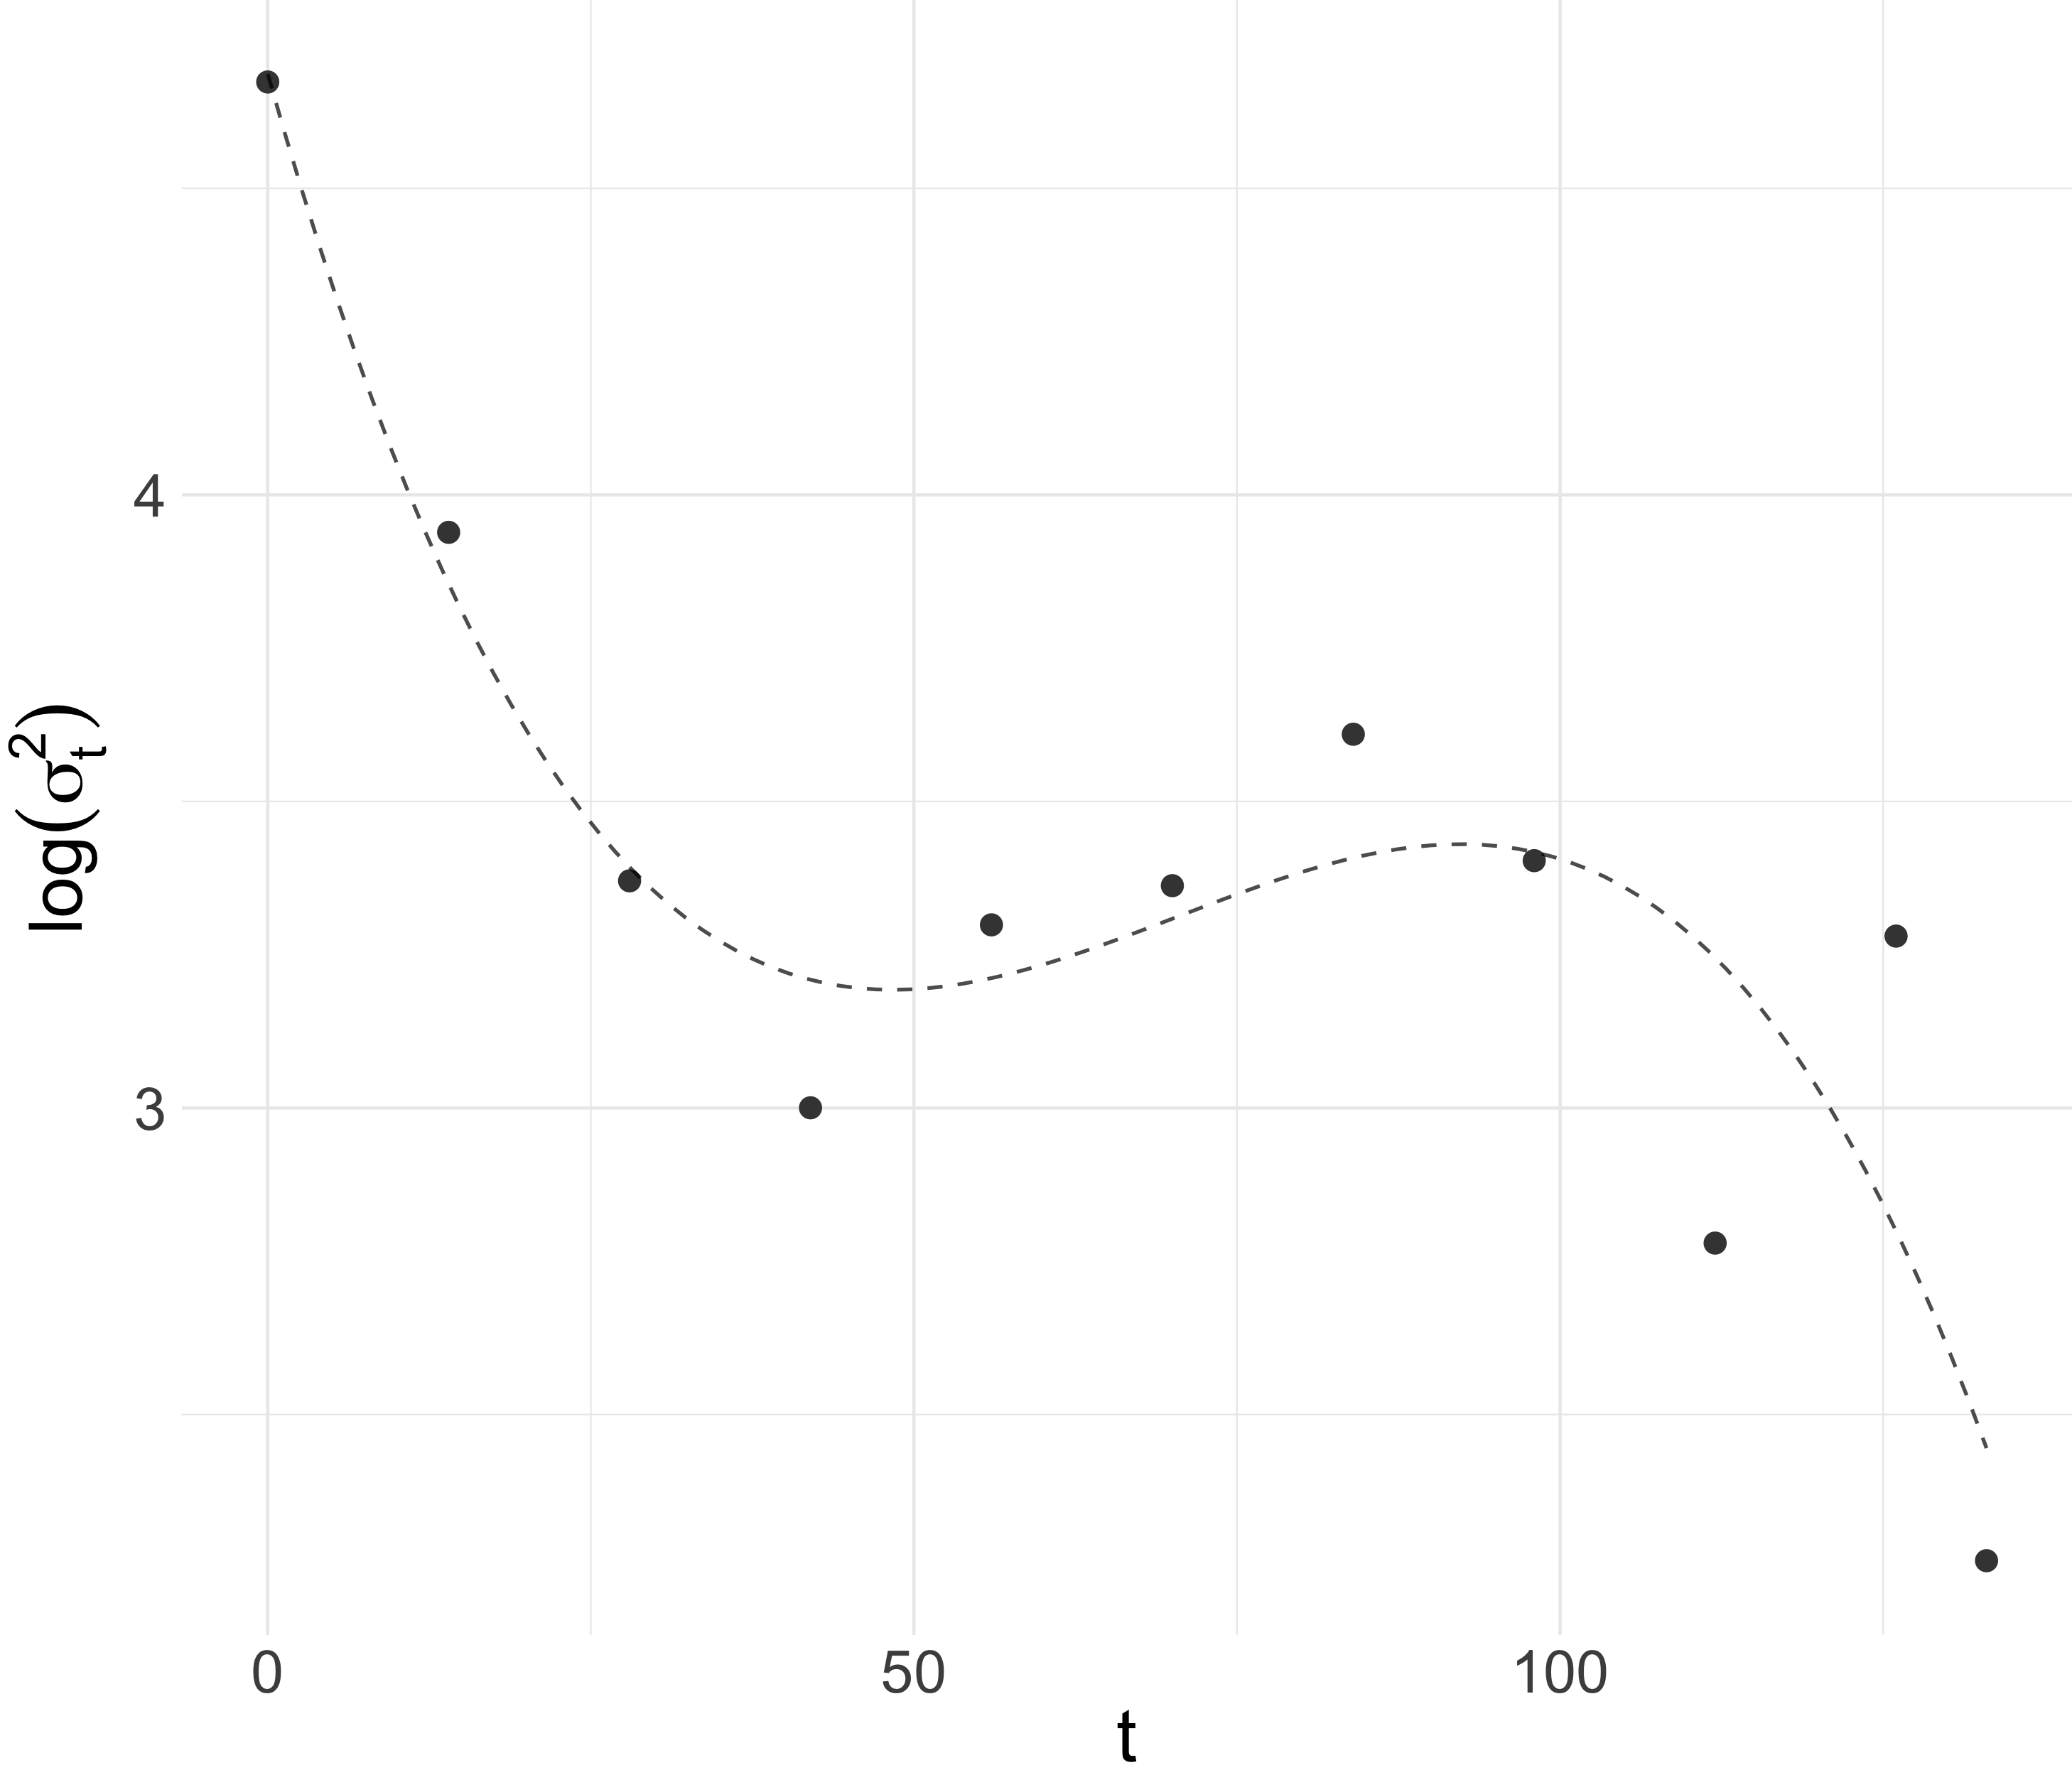
\includegraphics[width = \textwidth]{img/cattle/cattleA-innovariogram-with-cubic-smooth}
 \caption{\textit{Smoothed sample log innovation variances.} }
\label{fig:cattleA-innovariogram-with-cubic-smooth}
 \end{subfigure}
 \caption{\textit{Cubic polynomomials fitted to the sample regressogram and log innovation variances for the cattle data from treatment group A.}} \label{fig:cattleA-smoothed-regressogram-variogram}
\end{figure}


\bigskip


First things first: before estimating the covariance structure, we need to center the data using an adequate estimate of the mean weight trajectories. To account for any between-subject variability, we adopt an approach akin to the dynamical conditionally linear mixed model presented in \cite{pourahmadi2002dynamic}:

\begin{equation}
Y_i = f\left(t_i  \right) + Z_i b_i + \epsilon^*_i,
\end{equation} 

\noindent
where $Y_i$ is the $p_i \times 1$ response vector for the $i^{th}$ subject, $b_i$ is a $q \times 1$ vector of unknown random effects parameters, and $Z_i$ is a known $p_i \times q$ design matrix.  $f$ is the smooth function of $t$, and $t_i = \left(t_{i1}, \dots, t_{i,p_i}\right)'$ is the $p_i \times 1$ vector of measurement times for subject $i$. We specify the random term $Z_i b_i$ as an intercept only, letting $Z_i = \left(1 , \dots, 1\right)'$ so that 

\[
 Z_i b_i = \alpha_i 1_{p_i}, 
\] 

\noindent
so that the random effect corresponds to a subject-specific shift $\alpha_i$, which are assumed to be independent and identically distributed $N\left(0,\sigma_\alpha^2\right)$ random variables. We assume that the $p_i \times 1$ vector of residuals

\[
\epsilon^*_i \sim N\left(0, \Sigma_i\right).
\] 

\noindent
are mutually independent of the random intercepts $\alpha_i$, $i = 1,\dots, N$. Given that the animals belong to the same treatment group and share a common set of observation times, we assume each subject shares common covariance matrix $\Sigma_i = \Sigma$. We let $f$ belong to the Hilbert space

\[
\mathcal{C}^2 = \left\{f: \; f,\;f' \mbox{ absolutely continuous, } \int\left(f''\left(x\right)\right)^2 \;dx < \infty  \right\}. 
\]

\noindent
We take the estimators of $f$, $\alpha = \left(\alpha_1,\dots, \alpha_N\right)'$ to minimize the penalized joint log likelihood

\begin{equation}
\sum_{i = 1}^N \sum_{i = 1}^{p_i} \left(y_{ij} - f\left(t_{ij} \right) - \alpha_i \right)^2 + \alpha' \Sigma_\alpha^{-1} \alpha + \lambda J \left(f\right)
\end{equation}

\noindent
where $\textup{Cov}\left(\alpha\right) = \Sigma_\alpha = \sigma_\alpha^2 \mathrm{I}$. The variance of the random effects $\sigma^{-2}_\alpha$  is viewed as an additional smoothing parameter and estimated alongside $\lambda$. Figure~\ref{fig:cattleA-smoothed-weights-vs-time} shows the corresponding fitted mean curves. 

%Figure~\ref{fig:cattleA-weights-vs-time} displays the observed weight trajectories over time. 
%
%\begin{figure}[H] 
%\begin{center}
%    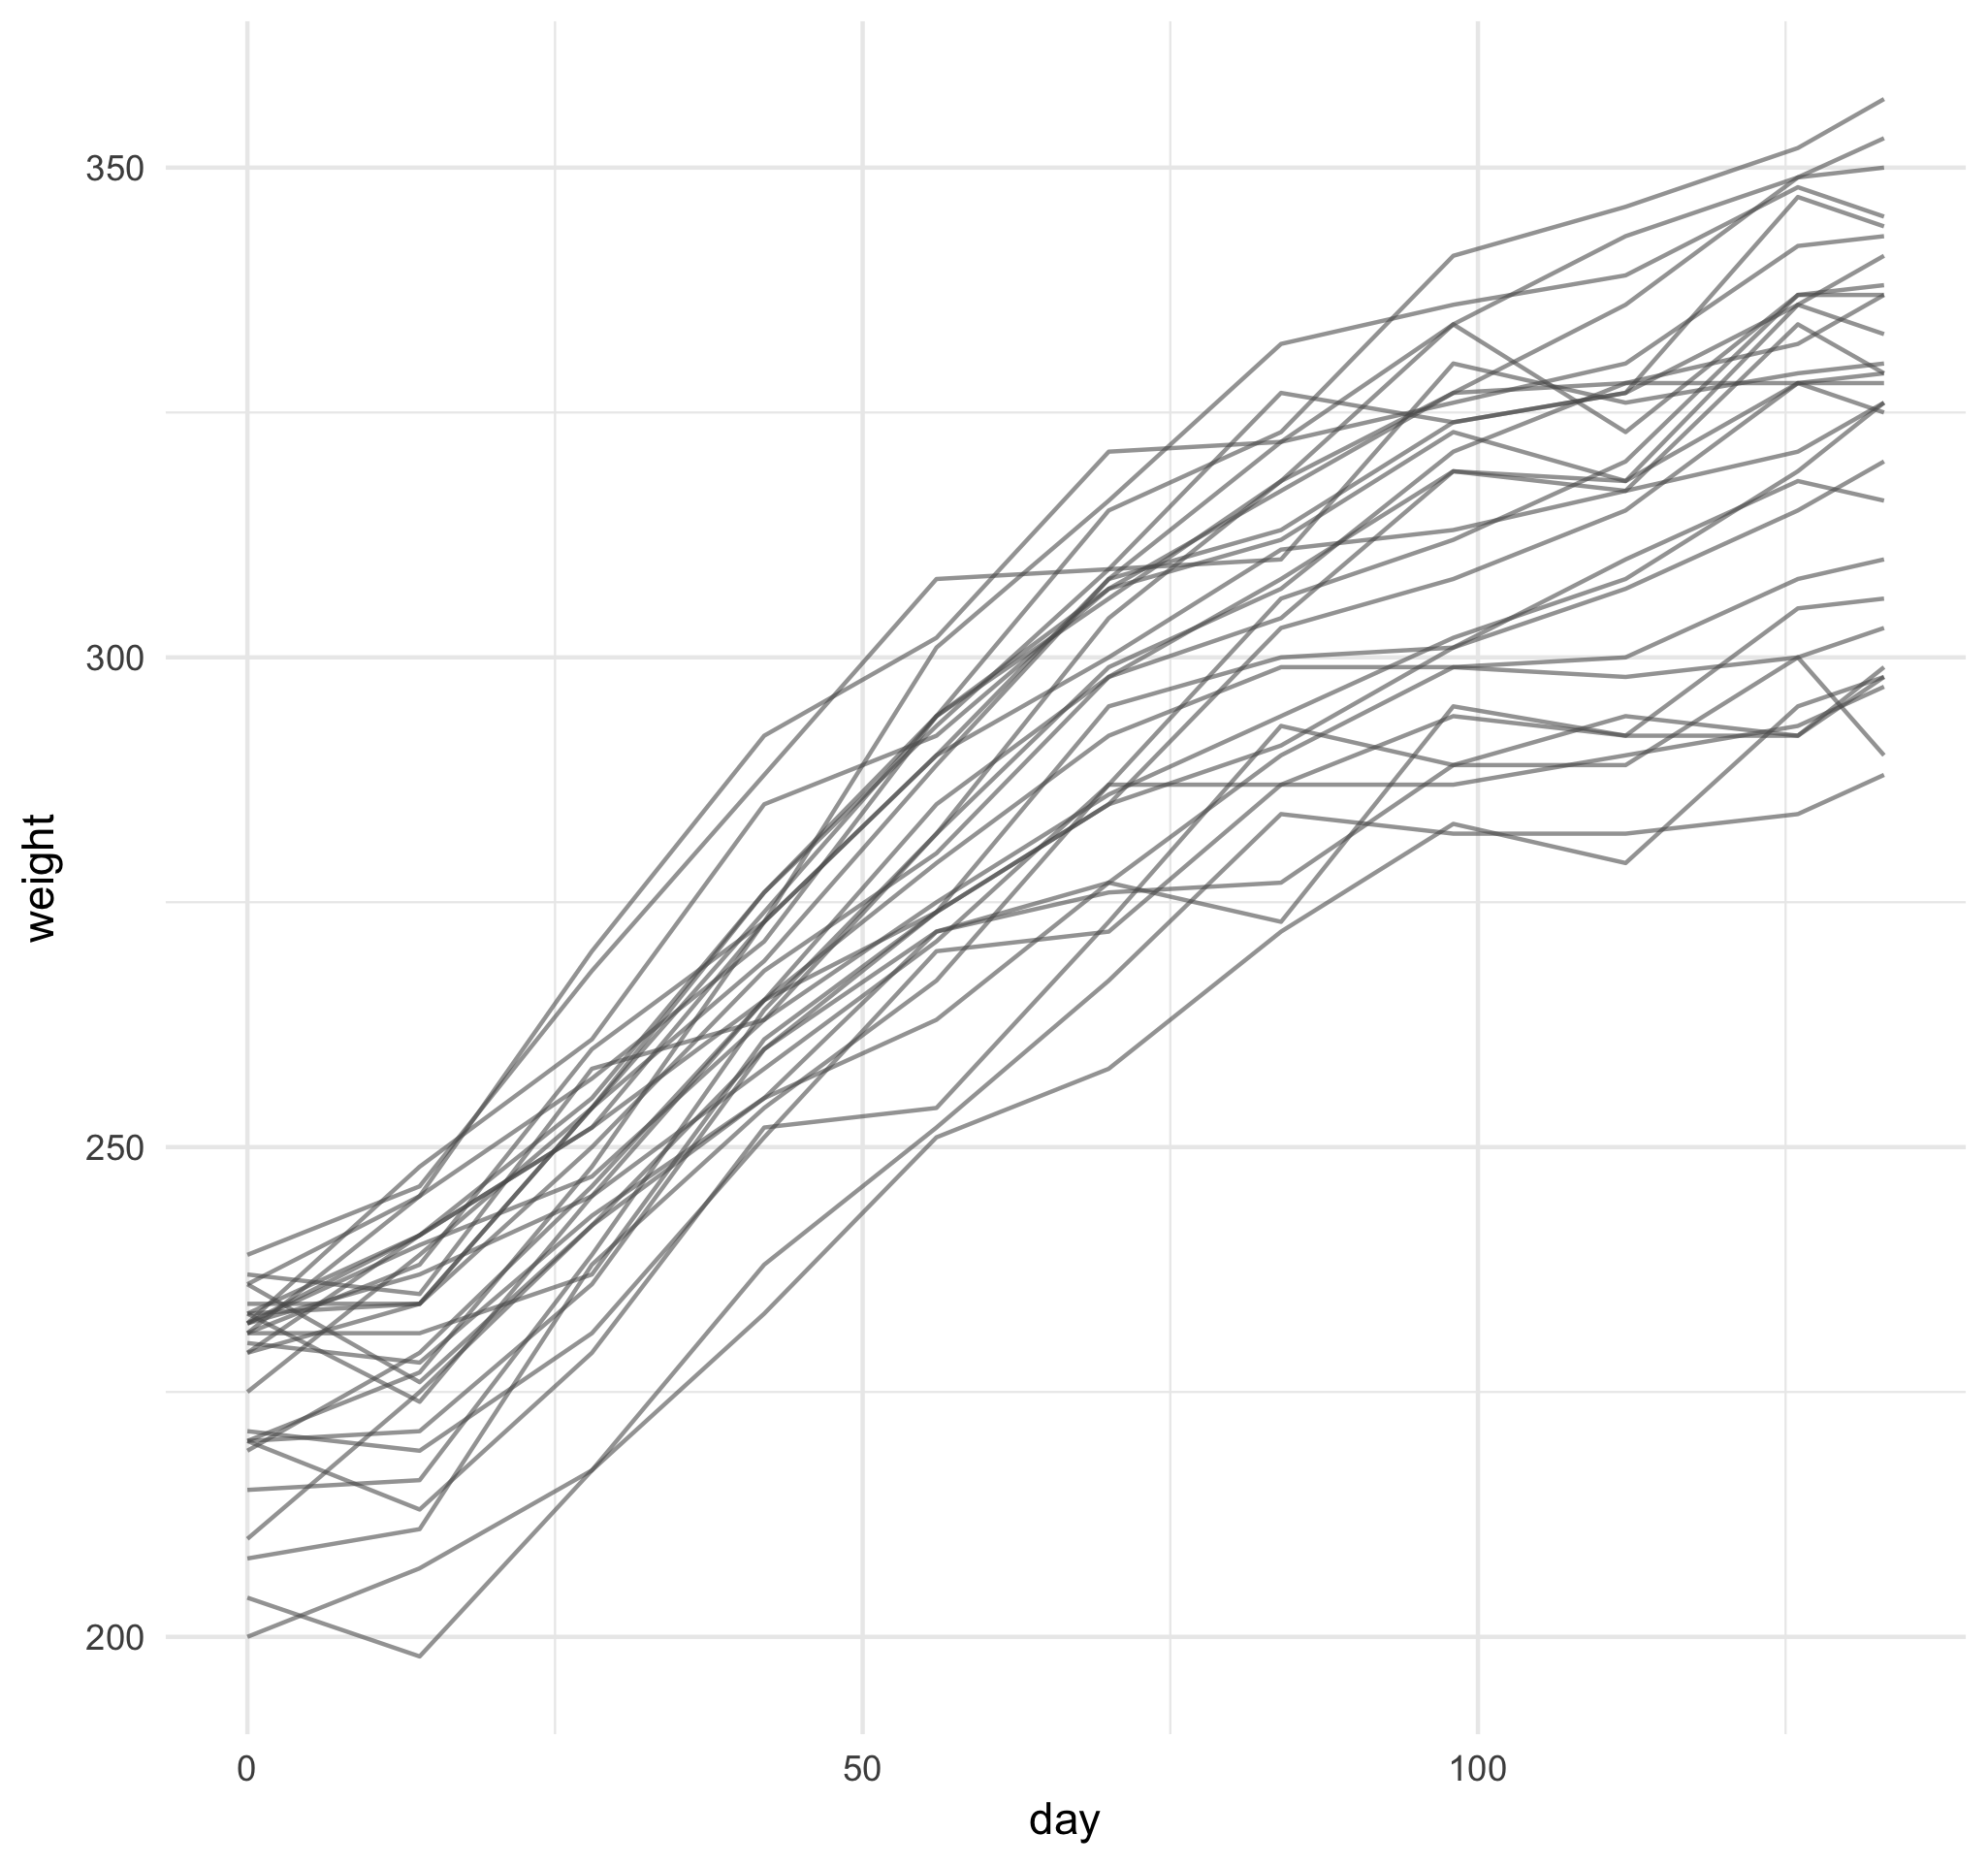
\includegraphics[width=.7\textwidth]{img/cattle/cattleA-weights-vs-time}
%\end{center}
% \caption{\textit{Weight trajectories over the observation period for experimental units in treatment group A.}}\label{fig:cattleA-weights-vs-time}
% \end{figure}

\begin{figure}[H] 
\begin{center}
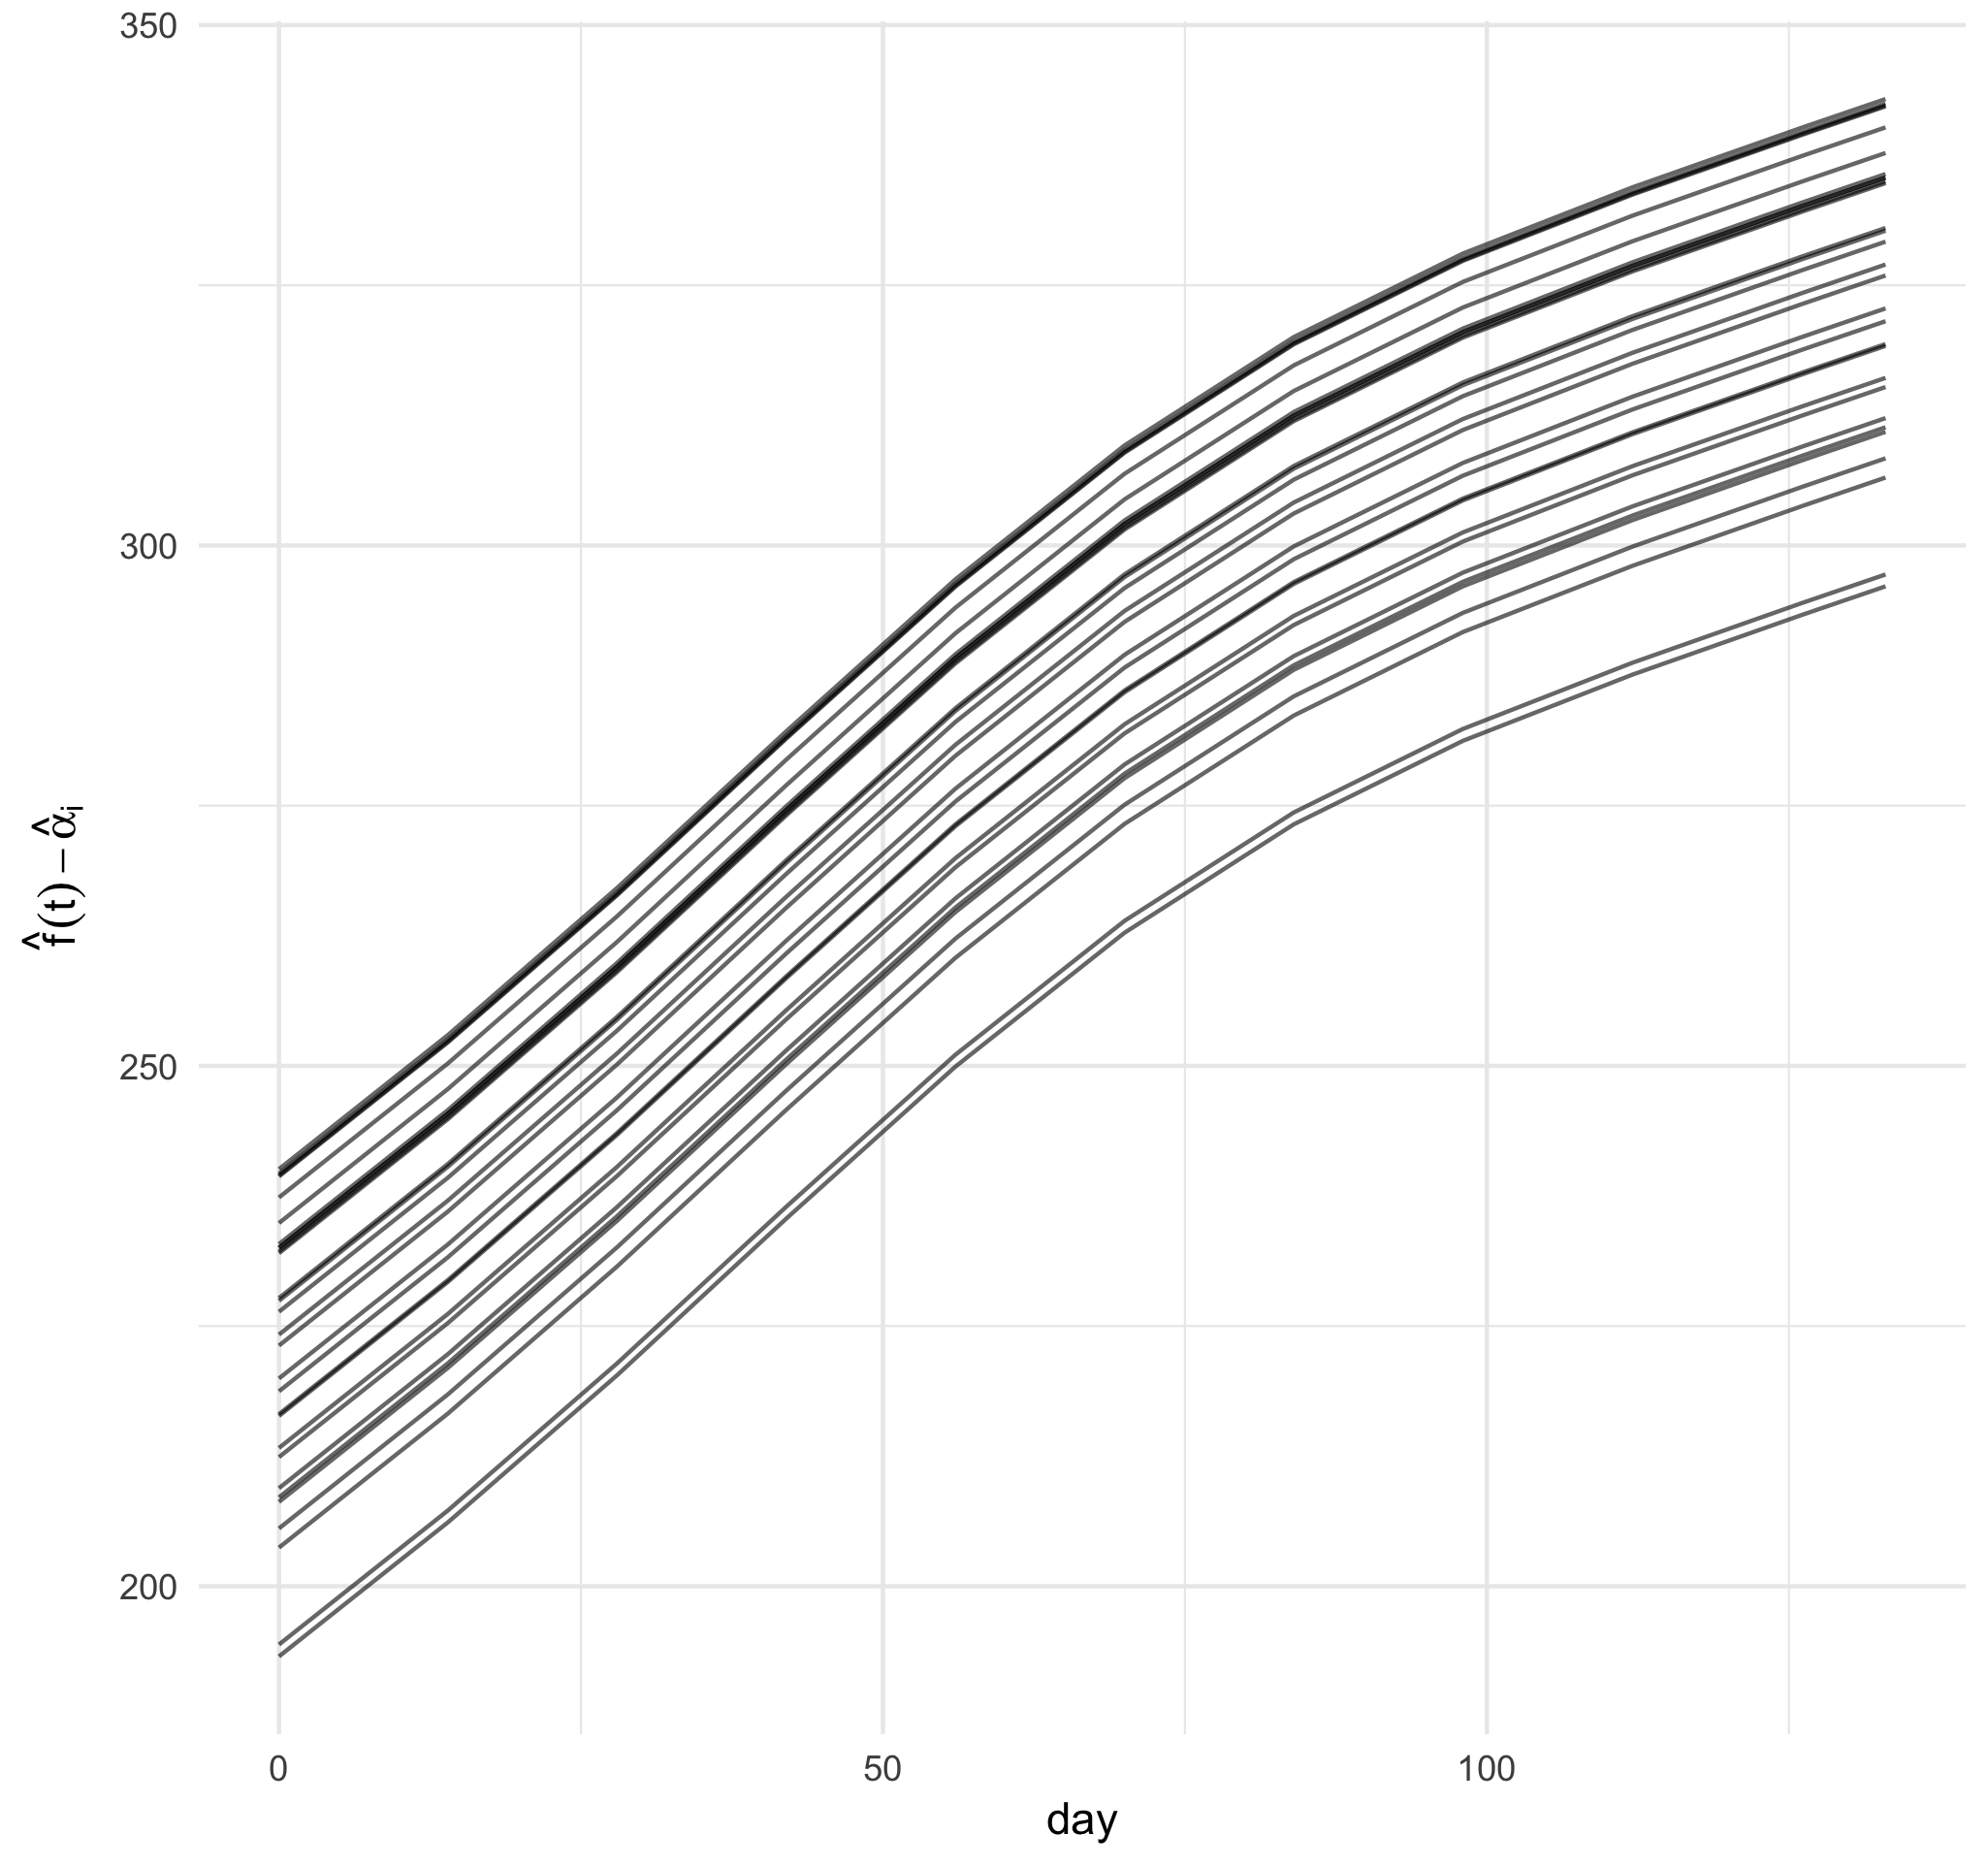
\includegraphics[width = .7\textwidth]{img/cattle/cattleA-weights-vs-time-mean-fit}
\caption{\textit{Subject-specific fitted weight trajectories for cattle in treatment group A. }}
\label{fig:cattleA-smoothed-weights-vs-time}
\end{center}
\end{figure} 

Centering the data using the fitted mean, the residuals 

\begin{equation} \label{eq:cattleA-dynamic-cond-mixed-model-2}
\epsilon^*\left(t_{ij}\right) = y\left(t_{ij}\right) - \left(f\left(t_{ij} \right) + \alpha_{i}\right).
\end{equation}

\noindent
serve as the data for estimating the functions defining the Cholesky factor and innovation variances. We model

\begin{equation} \label{eq:cattleA-dynamic-cond-mixed-model-1}
\epsilon^*\left(t_{ij}\right) = \sum_{k < j} \phi\left( t_{ij}, t_{ik} \right) \epsilon^*\left(t_{ij}\right) + \sigma\left(t_{ij}\right)\epsilon\left(t_{ij}\right).
\end{equation}

\noindent
where $\epsilon$ is a mean zero gaussian process with unit variance.

\bigskip

Choice of penalty is critical for convergence of the iterative estimation of $\phi$ and $\log\left(\sigma_2 \right)$. \cite{pan2017jmcm} concluded that the regressogram of empirical estimates of $\phi_{t,s}$ show consistent behaviour over $l = t - s$ for each value of $t$, indicating a lack of a strong functional component of $m$. This is consistent Pourahmadi's choice in the specification of model (\ref{eq:pourahmadi-cubic-model}) in terms of lag only. To balance the consideration of previous analyses with the interest of entirely data-driven model specification, we let $\phi \in \hilbert = \hilbert_{\left[1\right]} \otimes \hilbert_{\left[2\right]}$, where 

\begin{align*} 
\hilbert_{\left[1\right]} &= \bigg\{ \phi: \ddot{\phi} = 0 \bigg\} \oplus \left\{\phi: \phi\left(0\right) = \dot{\phi}\left(0\right) = 0; \;\; \int\limits_0^1 \ddot{\phi}^2 \;dx < \infty \right\} \\
\hilbert_{\left[2\right]} &= \bigg\{ \phi: \phi \propto 1 \bigg\} \oplus \left\{ \phi: \int\limits_0^1 \phi \;dx = 0, \;\; \dot{\phi} \in \mathcal{L}_2\left[0,1\right]  \right\} 
\end{align*} 

This decomposition leads to a null space comprised of functions of $l$ only, which is attractive because it coincides with the modeling assumptions made by $\phi$ \cite{pan2017jmcm}, \cite{huang2006covariance}, and \cite{wu2003nonparametric} for the same data set.  Figure~\ref{fig:fitted-cholesky-decomposition-cattle-date} shows the estimated Cholesky surface $\phi\left( t,s\right)$ and innovation variance function $\sigma^2\left(t\right)$ evaluated at $t =  0,14, 28,\dots,112, 126,133$ and the corresponding pairs of observation times $\left(t,s\right)$, $0 \le s < t \le 133$. Figure~\ref{fig:cattle-fitted-cholesky-ssanova} shows $\hat{\phi}$ decomposed into the functional components of its ANOVA decomposition.


%\begin{figure}[H]
%\centering
%\subfloat[The sample regressogram for the cattle data from treatment group A, overlaid with a cubic polynomial smooth.]{
%  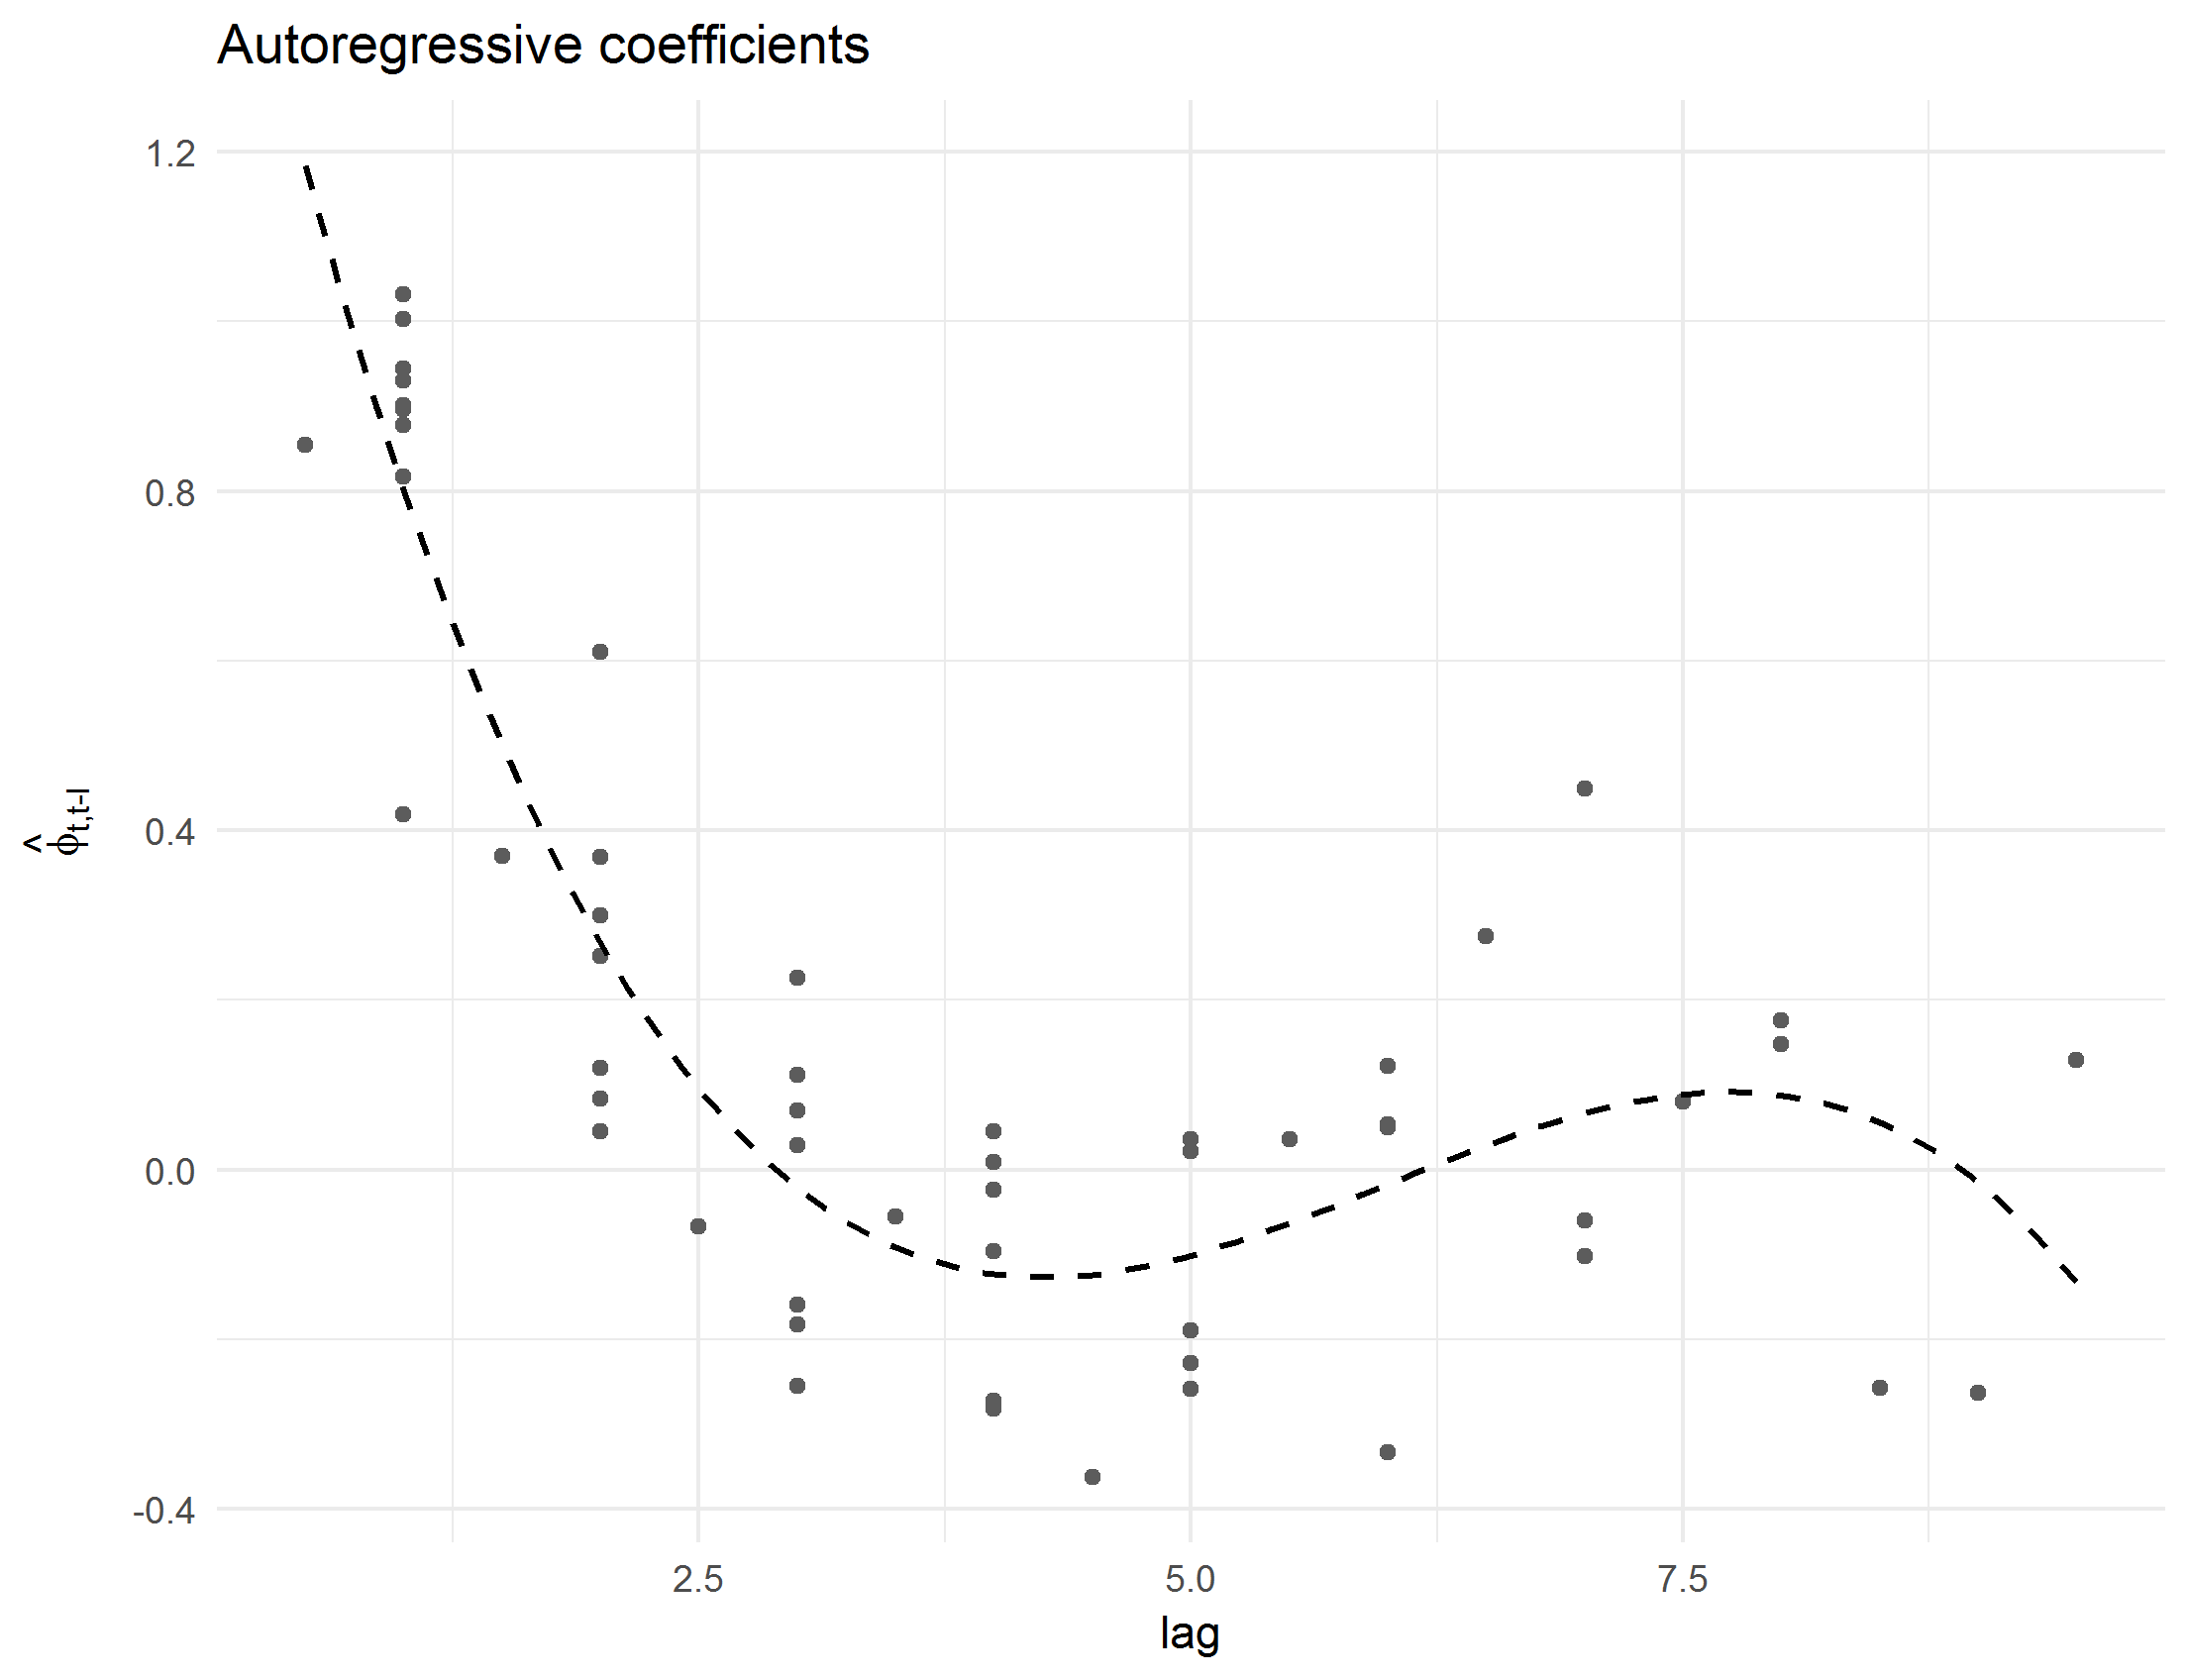
\includegraphics[width = .45\textwidth]{img/cattle/cattleA-regressogram-with-cubic-smooth}\label{fig:cattleA-regressogram-cubic-smooth}
%} 
%\hfill
%\subfloat[The sample variogram for the cattle data from treatment group A, overlaid with a cubic polynomial smooth.]{
%  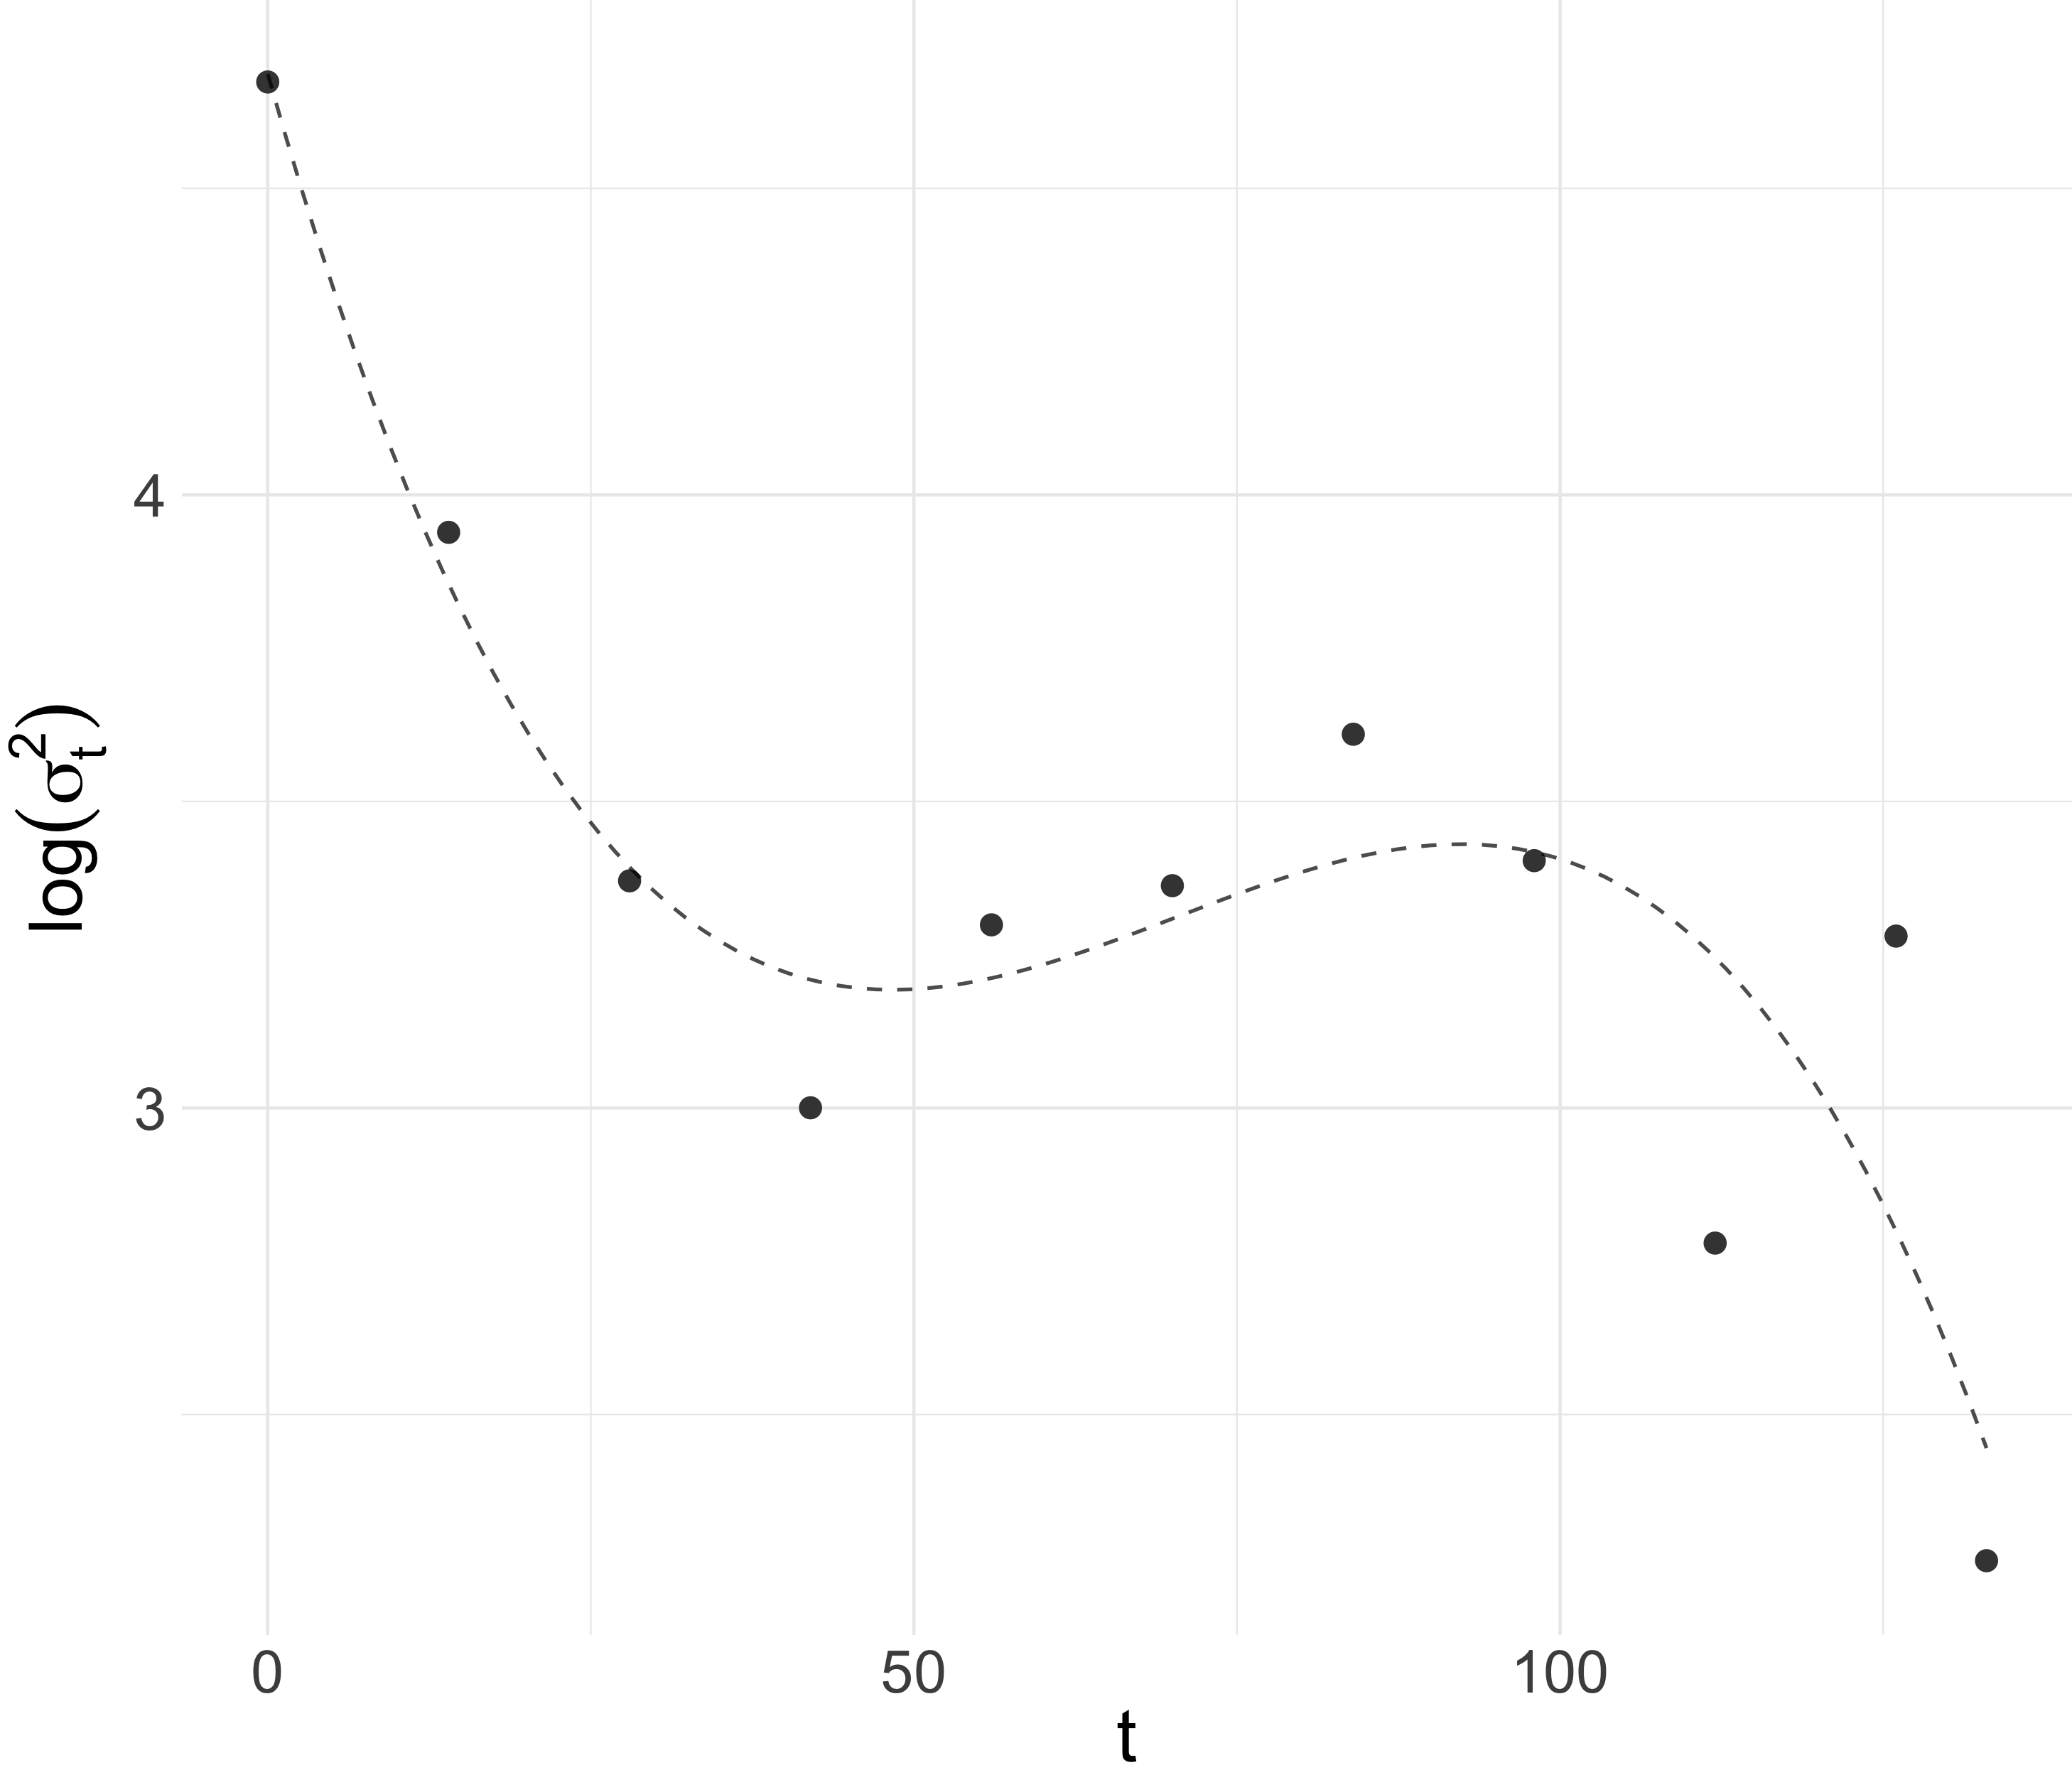
\includegraphics[width = .45\textwidth]{img/cattle/cattleA-innovariogram-with-cubic-smooth}\label{fig:cattleA-innovariogram-cubic-smooth}
%} 
%\end{figure}


%\begin{figure}[H]
% \begin{subfigure}{.33\textwidth}
%  \centering
%  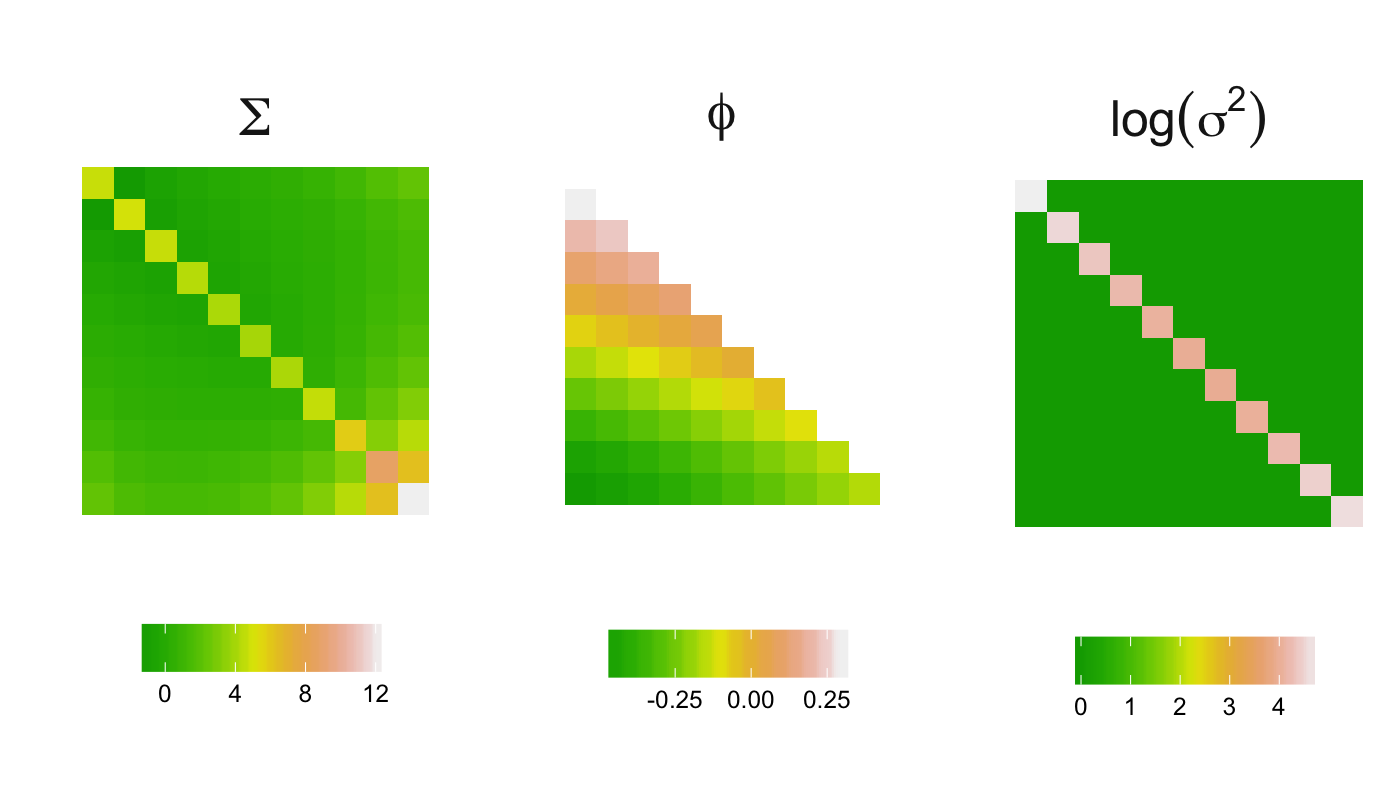
\includegraphics[width = \textwidth]{img/chapter-5/cattle-cholesky-estimate-ggplot}
% \caption{Estimated Cholesky factor $\hat{T}$}
% \end{subfigure}
% \begin{subfigure}{.33\textwidth}
%  \centering
%  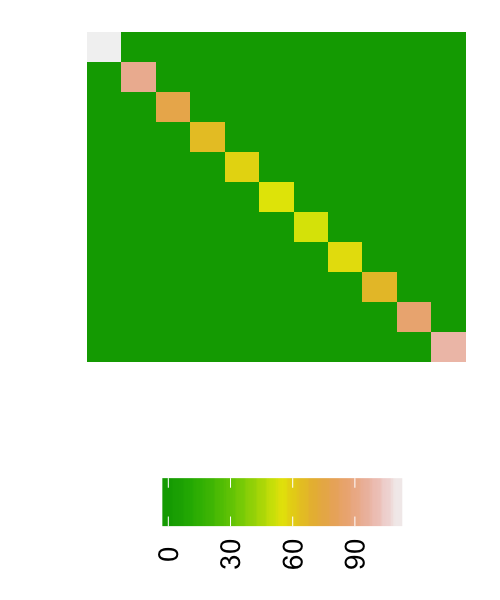
\includegraphics[width = \textwidth]{img/chapter-5/cattle-D-estimate-ggplot}
% \caption{Estimated innovation variances \newline $\hat{D} = diag\left( \sigma^2\left(t_1\right),\dots, \sigma^2\left(t_{11}\right) \right)$}
% \end{subfigure}
% \begin{subfigure}{.33\textwidth}
%  \centering
%  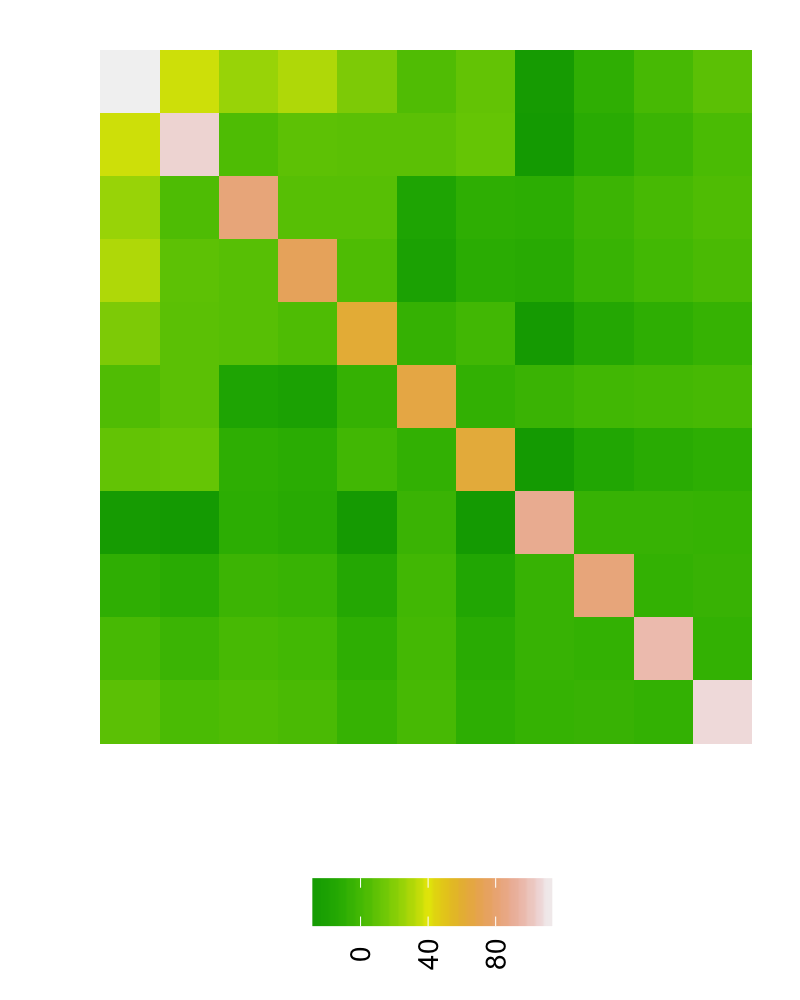
\includegraphics[width = \textwidth]{img/chapter-5/cattle-cov-estimate-ggplot}
% \caption{Estimated covariance matrix $\hat{\Sigma} = \hat{T}^{-1} \hat{D} {\hat{T}'}^{-1}$}
% \end{subfigure}
%\caption{Components of the fitted modified Cholesky decomposition for the cattle weight data.} \label{fig:fitted-cholesky-decomposition-cattle-date}
%\end{figure}
%
%
%\begin{figure}[H]
%  \centering
%  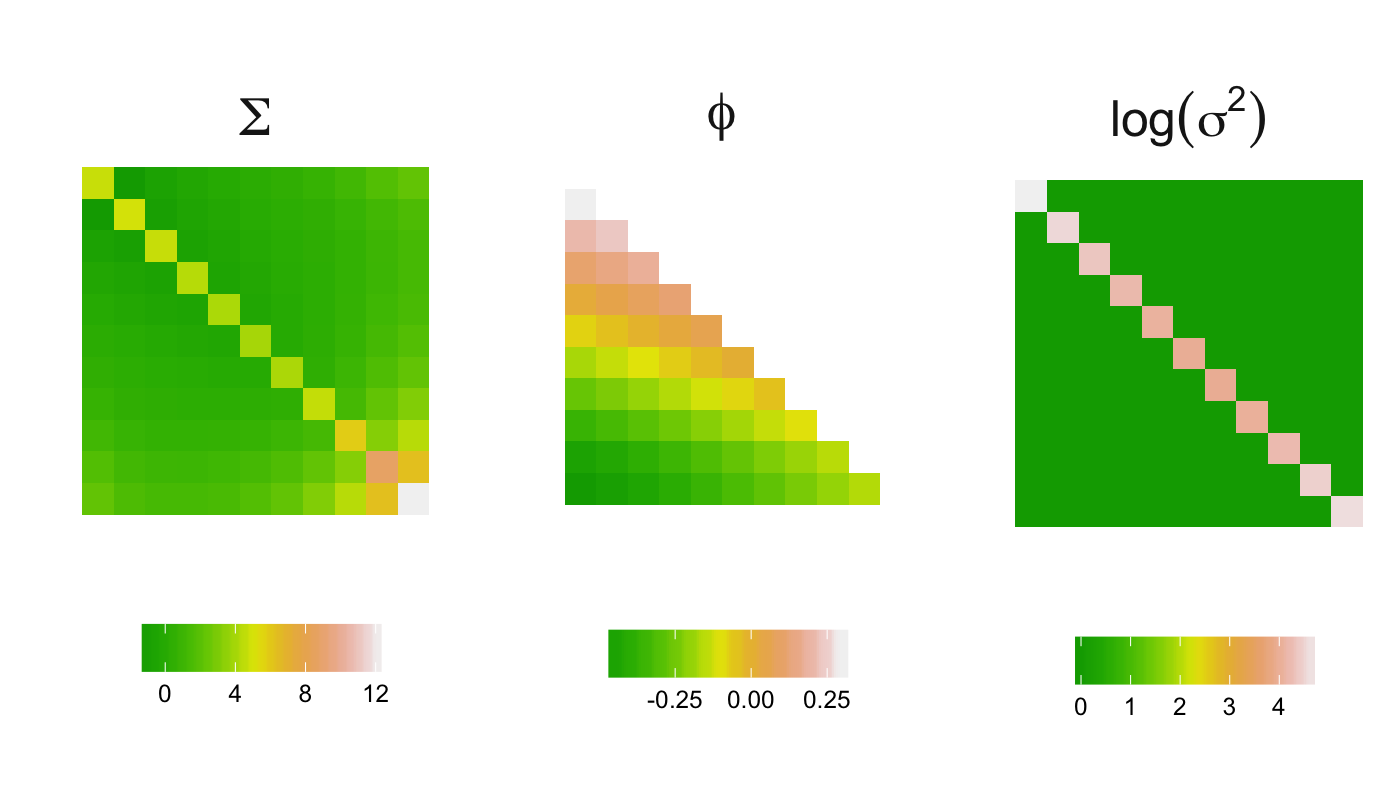
\includegraphics[width = \textwidth]{img/chapter-5/cattle-cholesky-estimate-ggplot}
%\caption{\textit{Components of the estimated covariance matrix for the cattle weight data from treatment group A: the sample covariance  }} \label{fig:fitted-cholesky-decomposition-cattle-date}
%\end{figure}

\begin{figure}[H]
 \begin{subfigure}[t]{.48\textwidth}
  \centering
  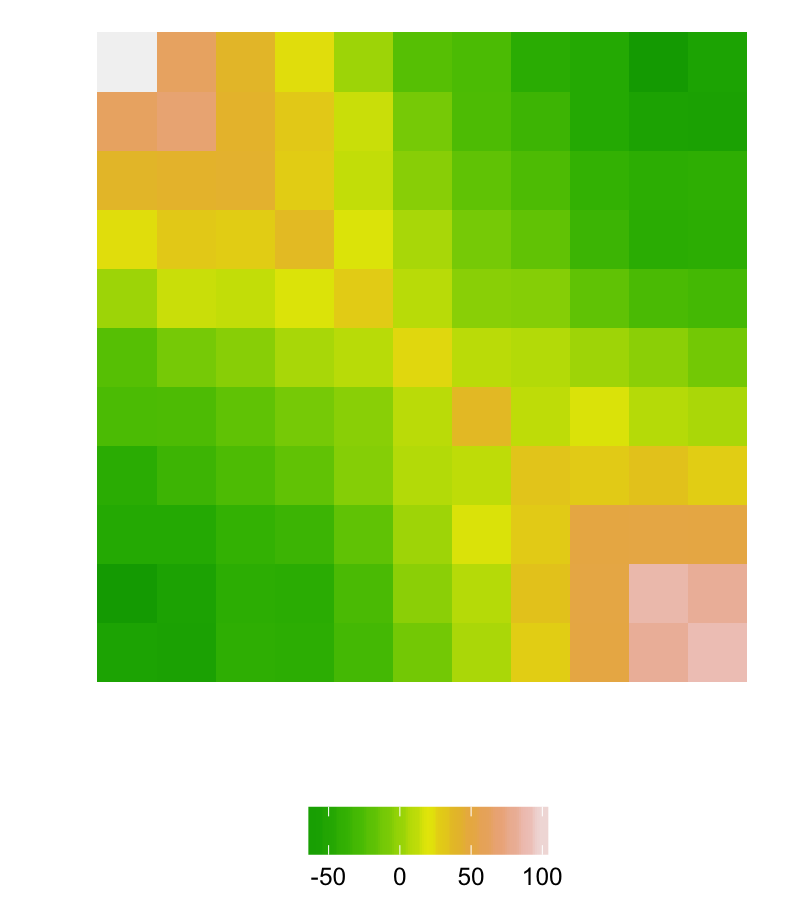
\includegraphics[width = \textwidth]{img/chapter-5/cattle-cholesky-estimate-ggplot-S}
 \caption{\textit{$S$}} \label{fig:fitted-cholesky-decomposition-cattle-date-S}
 \end{subfigure}
 \begin{subfigure}[t]{.48\textwidth}
  \centering
  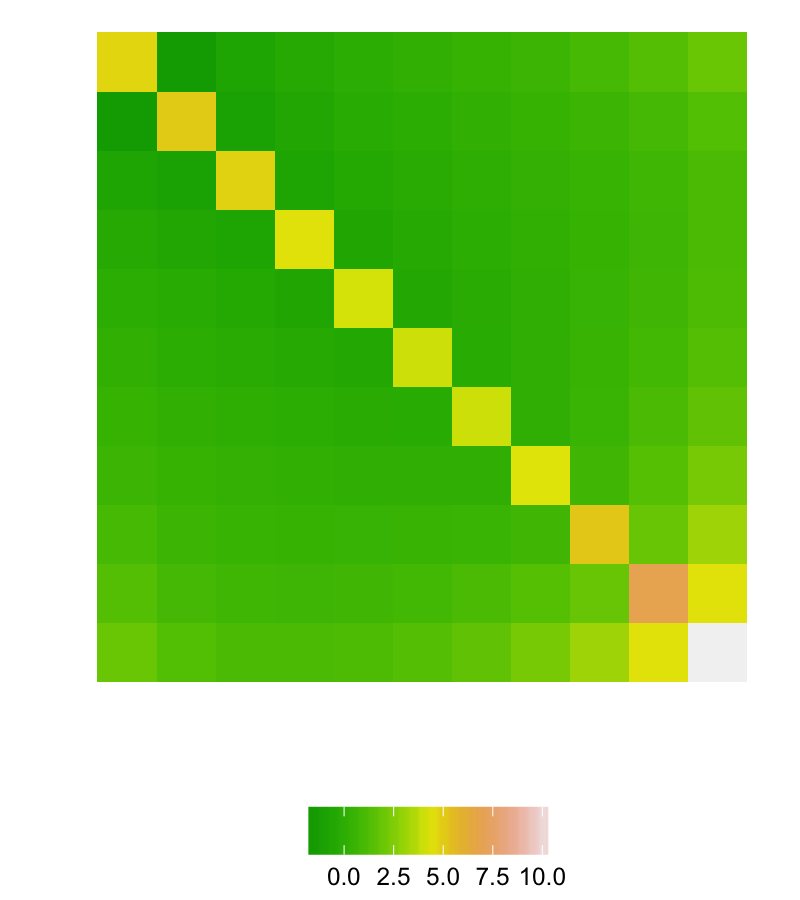
\includegraphics[width = \textwidth]{img/chapter-5/cattle-cholesky-estimate-ggplot-Sigma}
 \caption{\textit{ $\hat{\Sigma} = \hat{T}^{-1} \hat{D} \hat{T}'^{-1} $}}
\label{fig:fitted-cholesky-decomposition-cattle-date-Sigma}
 \end{subfigure}
  \begin{subfigure}[t]{.48\textwidth}
  \centering
  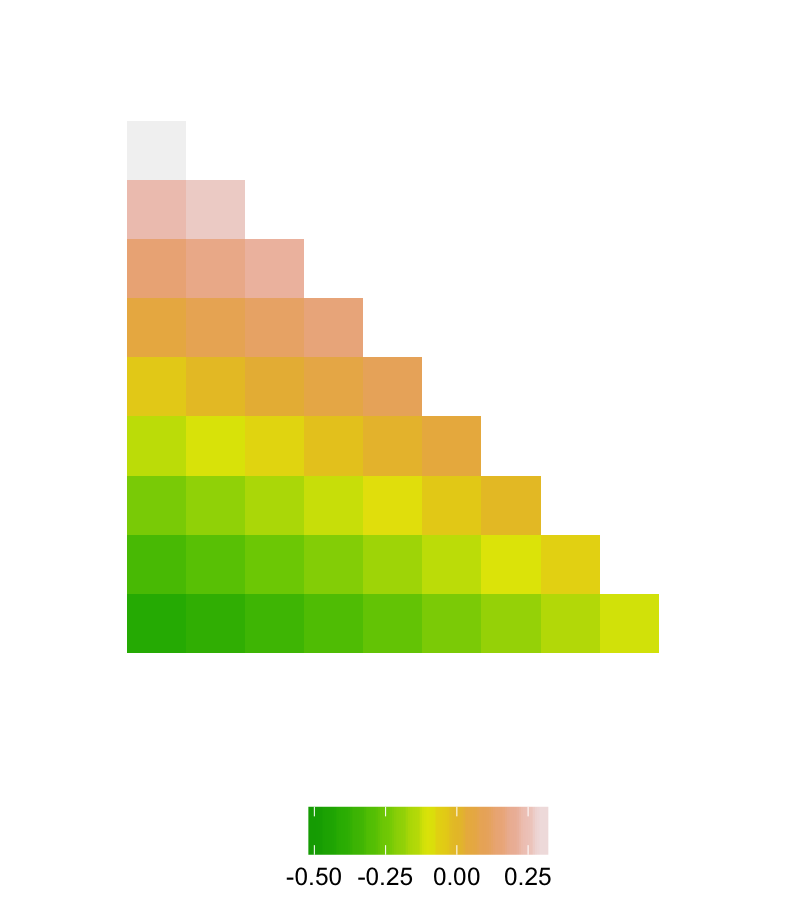
\includegraphics[width = \textwidth]{img/chapter-5/cattle-cholesky-estimate-ggplot-phi}
 \caption{\textit{$\hat{\phi}\left(t,s\right)$}} \label{fig:fitted-cholesky-decomposition-cattle-date-phi}
 \end{subfigure}
 \begin{subfigure}[t]{.48\textwidth}
  \centering
  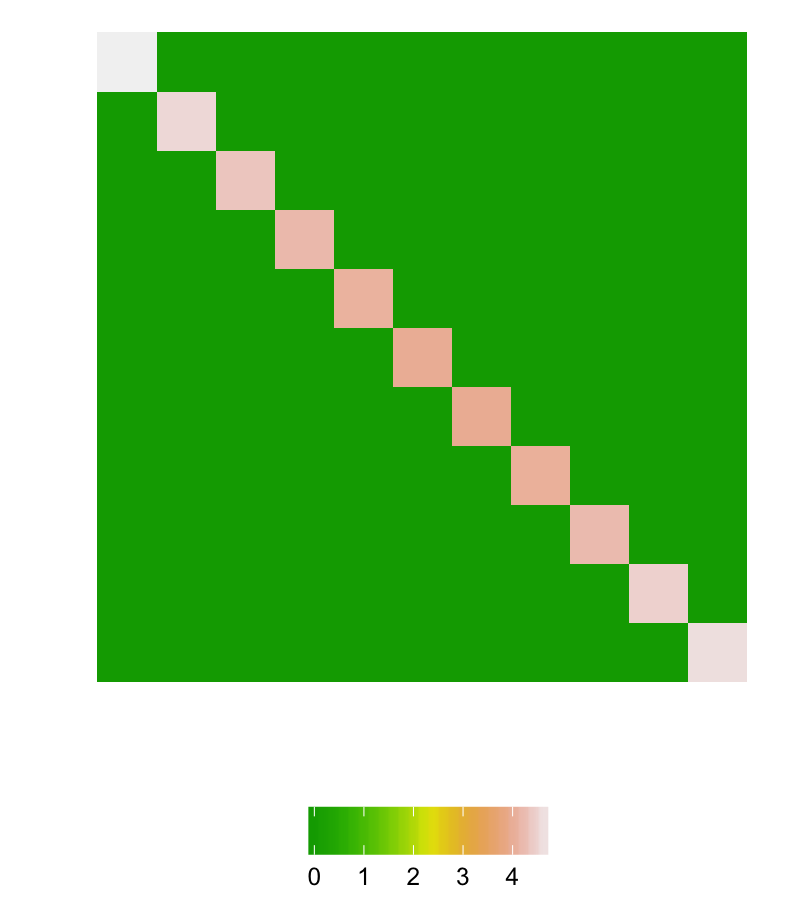
\includegraphics[width = \textwidth]{img/chapter-5/cattle-cholesky-estimate-ggplot-log-sigma2}
 \caption{\textit{$\hat{\sigma}^2\left(t\right)$}}
\label{fig:fitted-cholesky-decomposition-cattle-date-log-sigma2}
 \end{subfigure}
 \caption{\textit{The sample covariance matrix $S$, the estimated covariance matrix for the cattle weight data from treatment group A and the estimated Cholesky decomposition of the covariance matrix. The generalized autoregressive coefficient function $\phi\left(t,s\right)$ and the log innovation variances $\log \sigma^2\left(t\right)$ were estimated using a tensor product cubic spline and cubic spline, respectively. The fitted functions define the components of the Cholesky factor $\hat{T}$ and diagonal matrix $\hat{D}$.}}  \label{fig:fitted-cholesky-decomposition-cattle-date}
\end{figure}


%\subfile{chapter-5-subfiles/cattle-cholesky-ssanova-ggplot}
\begin{figure}[H] 
\centering
\caption{\textit{Components of the SSANOVA decomposition of the estimated generalized autoregressive coefficient function $\phi$ evaluated on the grid defined by the observed time points.}}
  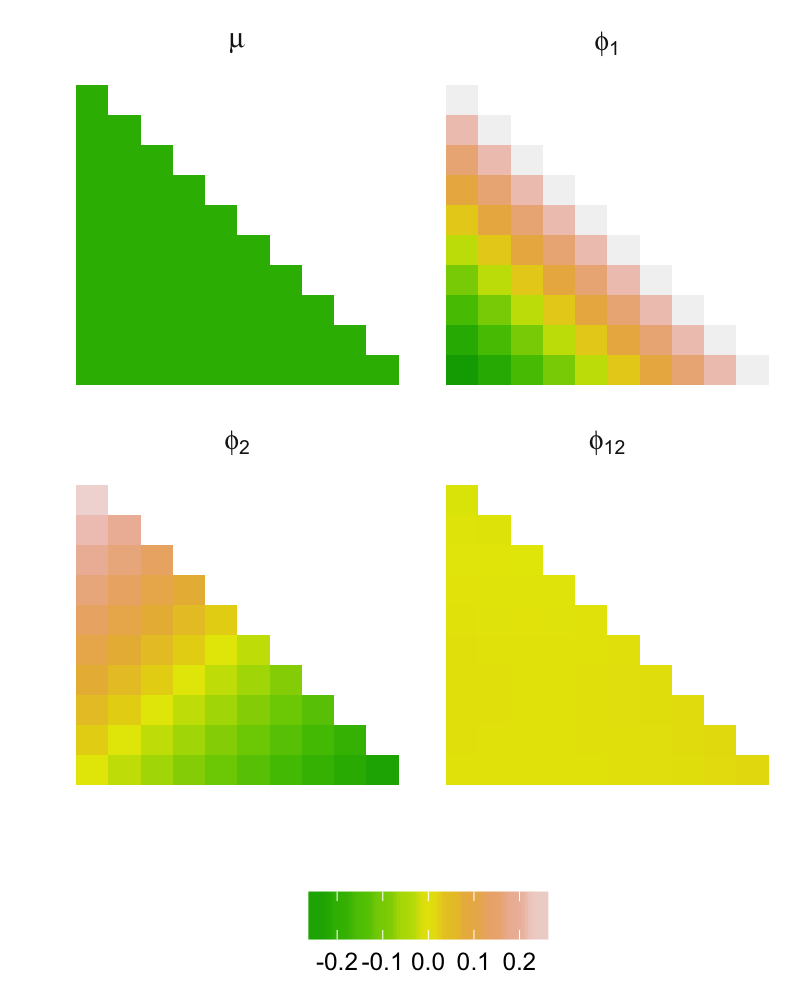
\includegraphics[width = 0.6\textwidth]{img/chapter-5/cattle-ssanova-estimate-lattice} \label{fig:cattle-fitted-cholesky-ssanova}
\end{figure}


Our sole focus on covariance estimation rather than the joint estimation of the mean and covariance makes apples-to-apples comparison with other analyses of the same dataset difficult. We constructed the mean estimate for the cattle in treatment group A shown in Figure~\ref{fig:cattleA-smoothed-weights-vs-time} entirely independently of the covariance estimate, which may be suboptimal compared to an iterative procedure that jointly estimates $f$, $b$, and $\Sigma$ as in \cite{pan2017jmcm} and \cite{pourahmadi1999joint}. Nevertheless, it is interesting to examine the differences between our estimates and cubic model fit shown in Figure~\ref{fig:cattleA-smoothed-regressogram-variogram}. Modeling $\phi$ as a polynomial in $l$ leaves any nonstationarity to be captured by the innovation variances. Of course, a model for the Cholesky factor having constant innovation variances and generalized autoregressive parameters which vary in $l$ only corresponds to a stationary process when certain conditions on the magnitude of the GARPs are satisfied (see \citep{klein1997statistical}, \citep{madsen2007time}). Our estimated model instead captures the non-stationarity with both the log innovation variances as well as with $\phi_2]$, the functional component corresponding to the main effect of $m$. The size of the functional components (in terms of the squared norm), however, does indicate a certain degree of concordance with the model proposed by \cite{pourahmadi1999joint}. The squared norm of the main effect of $l$, at 1.914, is over twice that of the main effect of $m$ (0.790), and the squared norm of the interaction term, as clearly indicated by Figure~\ref{fig:cattle-fitted-cholesky-ssanova}, is negligible in comparison to the main effects.

%Evaluating the normal likelihood at the fitted model gives $\hat{\ell} = -818.5323$.


%\bibliography{../Master}
%
%\end{document}
